\documentclass[12pt,a4paper]{article}

\usepackage[spanish]{babel}
\usepackage[T1]{fontenc}
\usepackage[utf8]{inputenc}
\usepackage[a4paper,margin=2.5cm]{geometry}
\usepackage{lmodern}
\usepackage{setspace}
\usepackage{hyperref}
\usepackage{amsmath,amssymb}
\usepackage{booktabs}
\usepackage{longtable}
\usepackage{enumitem}
\usepackage{graphicx}
\usepackage{caption}

\onehalfspacing
\hypersetup{
  colorlinks=true,
  linkcolor=black,
  urlcolor=black,
  pdfauthor={Juan Castello Beltran, Jaime Pérez Navarro y Hakan Hökelekli},
  pdftitle={Memoria tecnica del sistema recomendador de peliculas},
  pdfsubject={Sistemas Recomendadores},
  pdfkeywords={Recomendacion, Contenido, Colaborativo, Hibrido, Grupos, Evaluacion}
}

\graphicspath{{figures/}{screenshots/}}

\begin{document}
\pagenumbering{gobble}

\begin{titlepage}
\centering
{\Large Master en Inteligencia Artificial, Reconocimiento de Formas e Imagen Digital \par}
\vspace{2cm}
{\huge \bfseries Memoria tecnica del sistema recomendador de peliculas\par}
\vspace{0.8cm}
{\Large Sistemas Recomendadores\par}
\vfill
\begin{tabular}{ll}
Alumno: & Juan Castello Beltran \\
Fecha: & \today
\end{tabular}
\vfill
\end{titlepage}

\clearpage
\pagenumbering{arabic}
\tableofcontents
\newpage

\section{Introduccion}

El objetivo del trabajo es implementar una aplicacion completa de recomendacion de peliculas. La aplicacion permite obtener recomendaciones personalizadas para usuarios individuales y tambien para grupos, usando tres tecnicas: recomendacion basada en contenido, recomendacion colaborativa y recomendacion hibrida. El sistema se apoya en un dataset de peliculas y ratings, construye perfiles persistentes para los usuarios del dataset, permite crear nuevos usuarios desde la interfaz y evalua los recomendadores mediante metricas offline.

La idea central del sistema es calcular un ratio de interes usuario-pelicula y ordenar los items candidatos de mayor a menor puntuacion. Cada tecnica calcula ese ratio de una forma distinta. El recomendador basado en contenido compara el perfil del usuario con los metadatos de las peliculas; el colaborativo busca usuarios parecidos y predice ratings a partir de sus valoraciones; el hibrido combina ambas senales en una escala comun. Para los grupos, la aplicacion agrega recomendaciones individuales mediante estrategias de consenso.

La memoria se organiza siguiendo los bloques pedidos en la rubrica: tecnologias utilizadas, procesamiento de datos, interfaz, particion de ratings, funcionamiento de cada recomendador, recomendacion para grupos, evaluacion experimental y conclusiones.

\section{Tecnologia utilizada}

El proyecto esta desarrollado principalmente en Python. La parte de recomendacion y procesamiento de datos se implementa como modulos de backend, mientras que la interfaz grafica se construye en una aplicacion de escritorio con aspecto de aplicacion web mediante componentes visuales reutilizables.

\begin{itemize}[leftmargin=*]
\item \textbf{Python}: lenguaje principal del proyecto.
\item \textbf{pandas y numpy}: carga, limpieza y transformacion de datos.
\item \textbf{scikit-learn}: vectorizacion TF-IDF, codificacion de generos y calculo de similitudes.
\item \textbf{scipy}: almacenamiento disperso de la matriz usuario-genero del colaborativo.
\item \textbf{matplotlib}: generacion de graficas de evaluacion.
\item \textbf{openpyxl}: exportacion de resultados de evaluacion a Excel.
\item \textbf{aiohttp}: enriquecimiento asincrono del catalogo con datos de TMDb.
\item \textbf{JSON}: persistencia de peliculas procesadas, ratings y perfiles de usuario.
\end{itemize}

La organizacion del repositorio separa los componentes principales:

\begin{itemize}[leftmargin=*]
\item \texttt{Backend/}: algoritmos de recomendacion, gestion de usuarios y recomendacion de grupos.
\item \texttt{Frontend/}: interfaz de usuario, pantallas y servicios de datos.
\item \texttt{Data/Raw\_data/}: ficheros originales del dataset.
\item \texttt{Data/Clean\_data/}: datos procesados, enriquecidos y particionados.
\item \texttt{scripts/data/}: scripts de limpieza, particion e inicializacion.
\item \texttt{scripts/evaluation/}: evaluacion offline y generacion de metricas.
\item \texttt{docs/}: documentacion tecnica, memoria, capturas y graficas.
\end{itemize}

\section{Procesamiento de datos}

\subsection{Fuentes del dataset}

El sistema parte de varios ficheros ubicados en \texttt{Data/Raw\_data/}. Los mas importantes son:

\begin{itemize}[leftmargin=*]
\item \texttt{peliculas.csv}, con la informacion base del catalogo.
\item \texttt{ratings\_small.csv}, con las puntuaciones explicitas de los usuarios.
\item \texttt{keywords.csv}, con palabras clave asociadas a peliculas.
\item \texttt{generos.csv}, con el mapeo entre identificadores de genero y nombres legibles.
\item \texttt{links.csv}, con identificadores externos.
\end{itemize}

A partir de estos ficheros se generan varios artefactos en \texttt{Data/Clean\_data/}: \texttt{cleaned\_movies.json}, \texttt{cleaned\_ratings.json}, \texttt{train\_ratings.json}, \texttt{test\_ratings.json} y \texttt{enhanced\_movies.json}. Estos ficheros son la base comun de los tres recomendadores.

\subsection{Limpieza del catalogo y ratings}

Durante la limpieza se eliminan ratings cuyo \texttt{movieId} no aparece en el catalogo final. Esta decision es importante porque el enunciado advierte que algunas peliculas puntuadas pueden haber sido eliminadas del fichero de peliculas. Mantener esos ratings produciria comparaciones injustas: el usuario podria haber valorado una pelicula que el recomendador ya no puede recomendar ni mostrar.

Tambien se normalizan campos de peliculas, generos y keywords. Las keywords se extraen recorriendo las columnas utiles del fichero original, descartando valores vacios y construyendo una lista compacta por pelicula. Esta informacion se usa posteriormente en el recomendador basado en contenido.

\subsection{Enriquecimiento con TMDb}

El fichero \texttt{enhanced\_movies.json} amplia la informacion original de las peliculas mediante consultas a TMDb. Se incorporan campos como \texttt{overview}, \texttt{tagline}, \texttt{runtime}, \texttt{release\_date}, \texttt{poster\_path}, \texttt{backdrop\_path}, popularidad, valoracion media, votos, productoras, idiomas y colecciones.

Este enriquecimiento tiene dos ventajas. En la interfaz permite mostrar carteles y datos mas informativos. En el algoritmo de contenido aporta texto y metadatos semanticos que ayudan a diferenciar peliculas que comparten generos pero tratan temas distintos.

\subsection{Particion entrenamiento-test}

Los ratings limpios se dividen en entrenamiento y test con una proporcion 70\%-30\%. La particion se realiza por usuario, no de forma global. Para cada usuario se barajan sus ratings con semilla fija y se separa el 70\% para entrenamiento y el 30\% para evaluacion. Si un usuario tiene una unica valoracion, se conserva en entrenamiento para evitar perfiles vacios.

Esta particion evita fuga de informacion. Los perfiles, vecinos y recomendaciones se construyen con \texttt{train\_ratings.json}; las metricas se calculan comparando las recomendaciones contra \texttt{test\_ratings.json}.

\subsection{Registro de usuarios}

El fichero \texttt{Data/user\_registry.json} almacena el perfil persistente de cada usuario. Para los usuarios del dataset se genera a partir del conjunto de entrenamiento. Cada entrada incluye el identificador, estado, tipo de usuario, peliculas vistas, ratings agregados, generos favoritos y un vector de preferencias por genero.

El vector de generos se obtiene a partir de las peliculas puntuadas por el usuario. Para cada rating se compara la puntuacion con la media personal del usuario:

\[
weight = rating - media\_usuario
\]

Si una pelicula esta por encima de la media del usuario, sus generos reciben una contribucion positiva. Si esta por debajo, reciben una contribucion menor o negativa. Finalmente, el vector se normaliza al rango $[0,100]$. Asi, el perfil no refleja solo que generos ha visto el usuario, sino que generos ha valorado mejor respecto a su propio criterio.

Para nuevos usuarios, la interfaz permite seleccionar generos favoritos. Con esa informacion se inicializa un perfil basico que permite recomendar desde el primer uso, reduciendo el problema de \emph{cold start}.

\section{Interfaz y funcionamiento}

La interfaz permite autenticar usuarios, explorar el catalogo, consultar estadisticas, valorar peliculas, crear nuevos usuarios, obtener recomendaciones individuales y generar recomendaciones para grupos. Las capturas incluidas en esta seccion muestran el flujo principal de uso.

\begin{figure}[htbp]
\centering
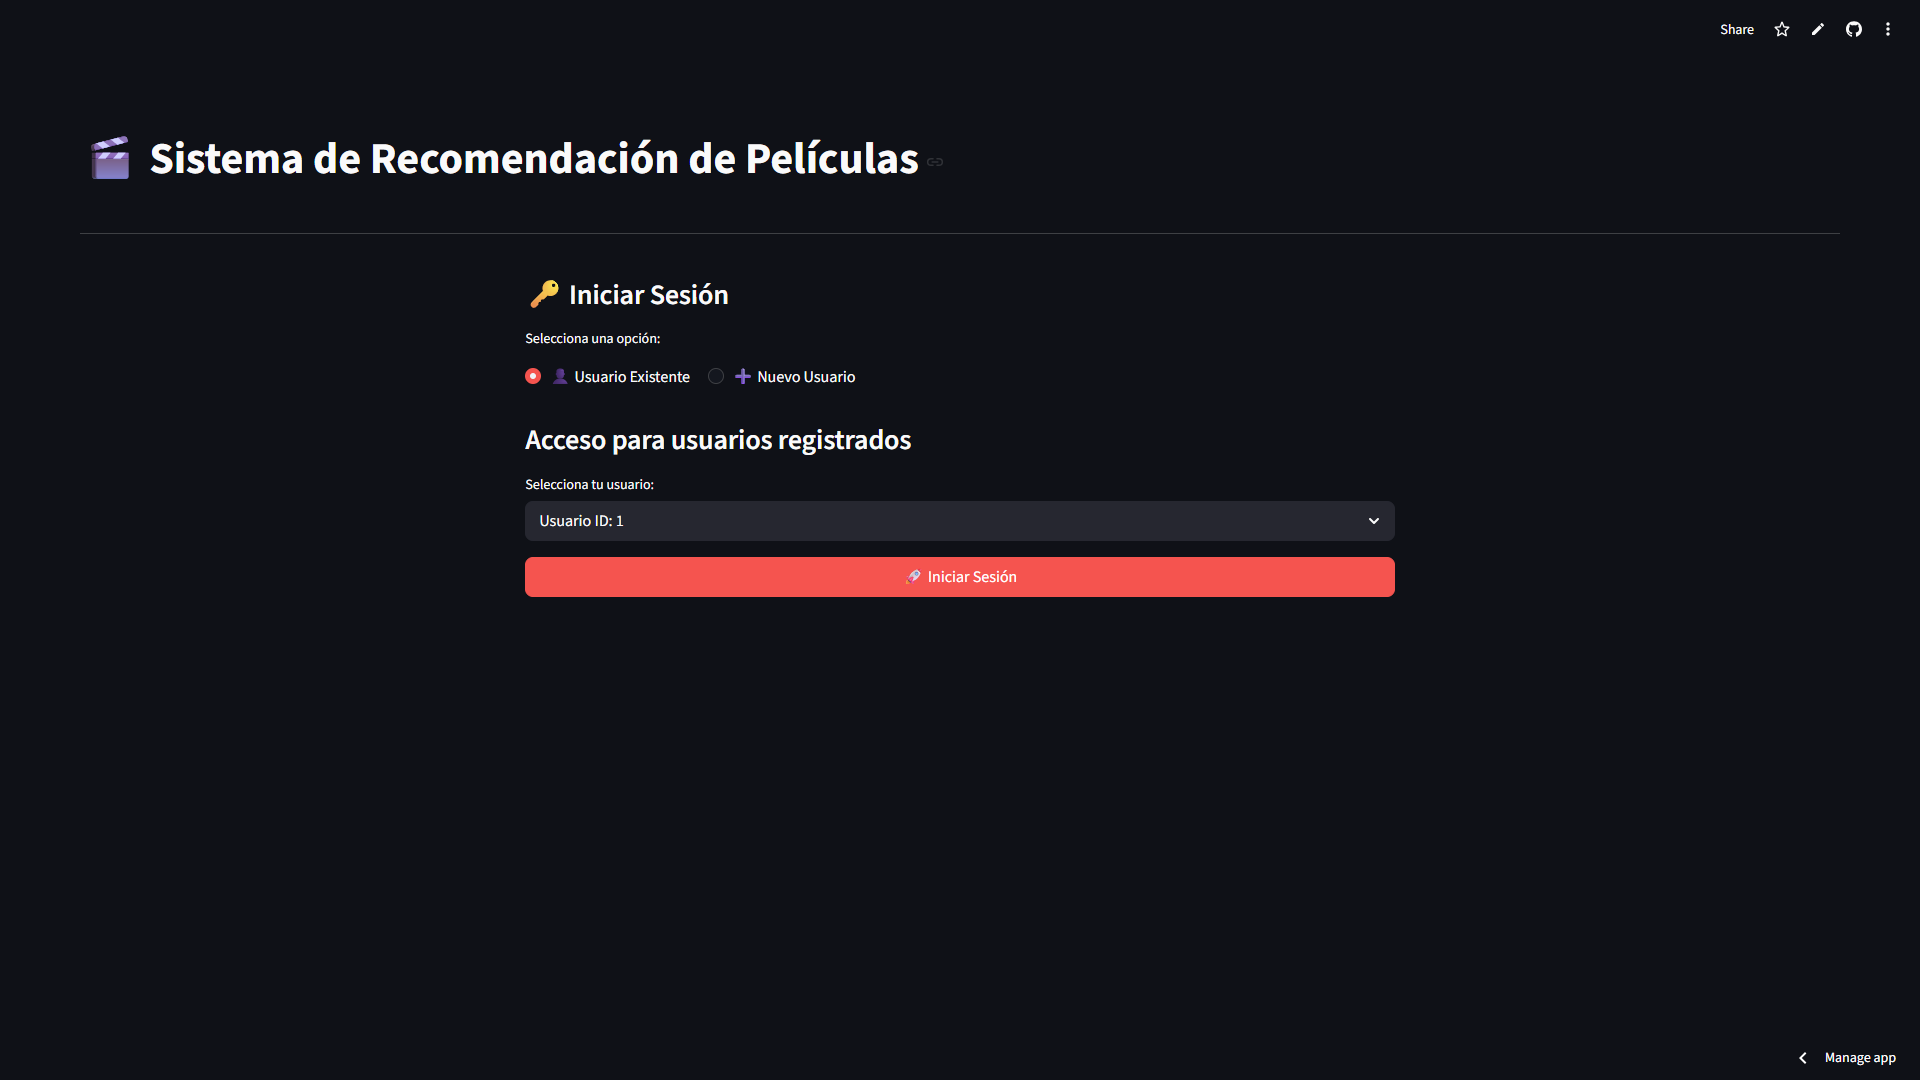
\includegraphics[width=0.82\textwidth]{Login.png}
\caption{Pantalla de acceso a la aplicacion.}
\end{figure}

\begin{figure}[htbp]
\centering
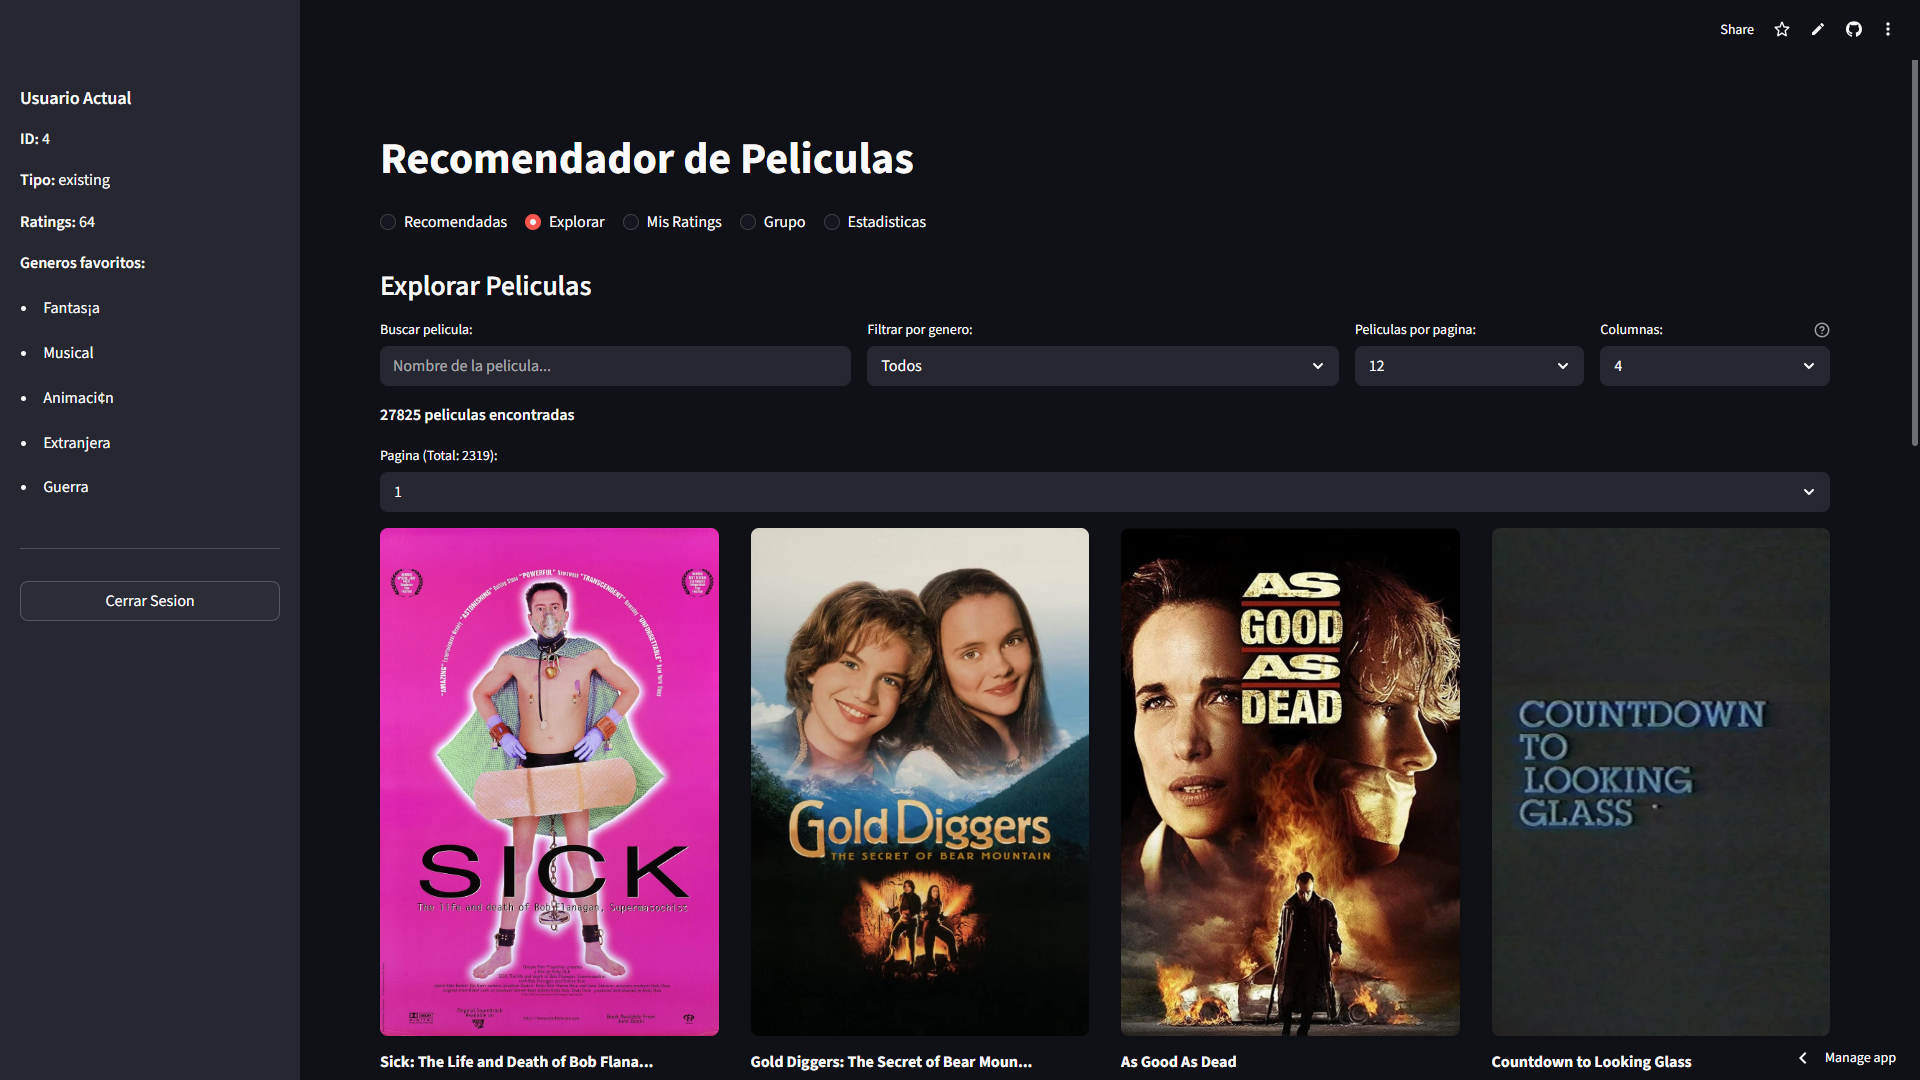
\includegraphics[width=0.95\textwidth]{HomePage_explore_windows.png}
\caption{Vista principal de exploracion del catalogo.}
\end{figure}

\begin{figure}[htbp]
\centering
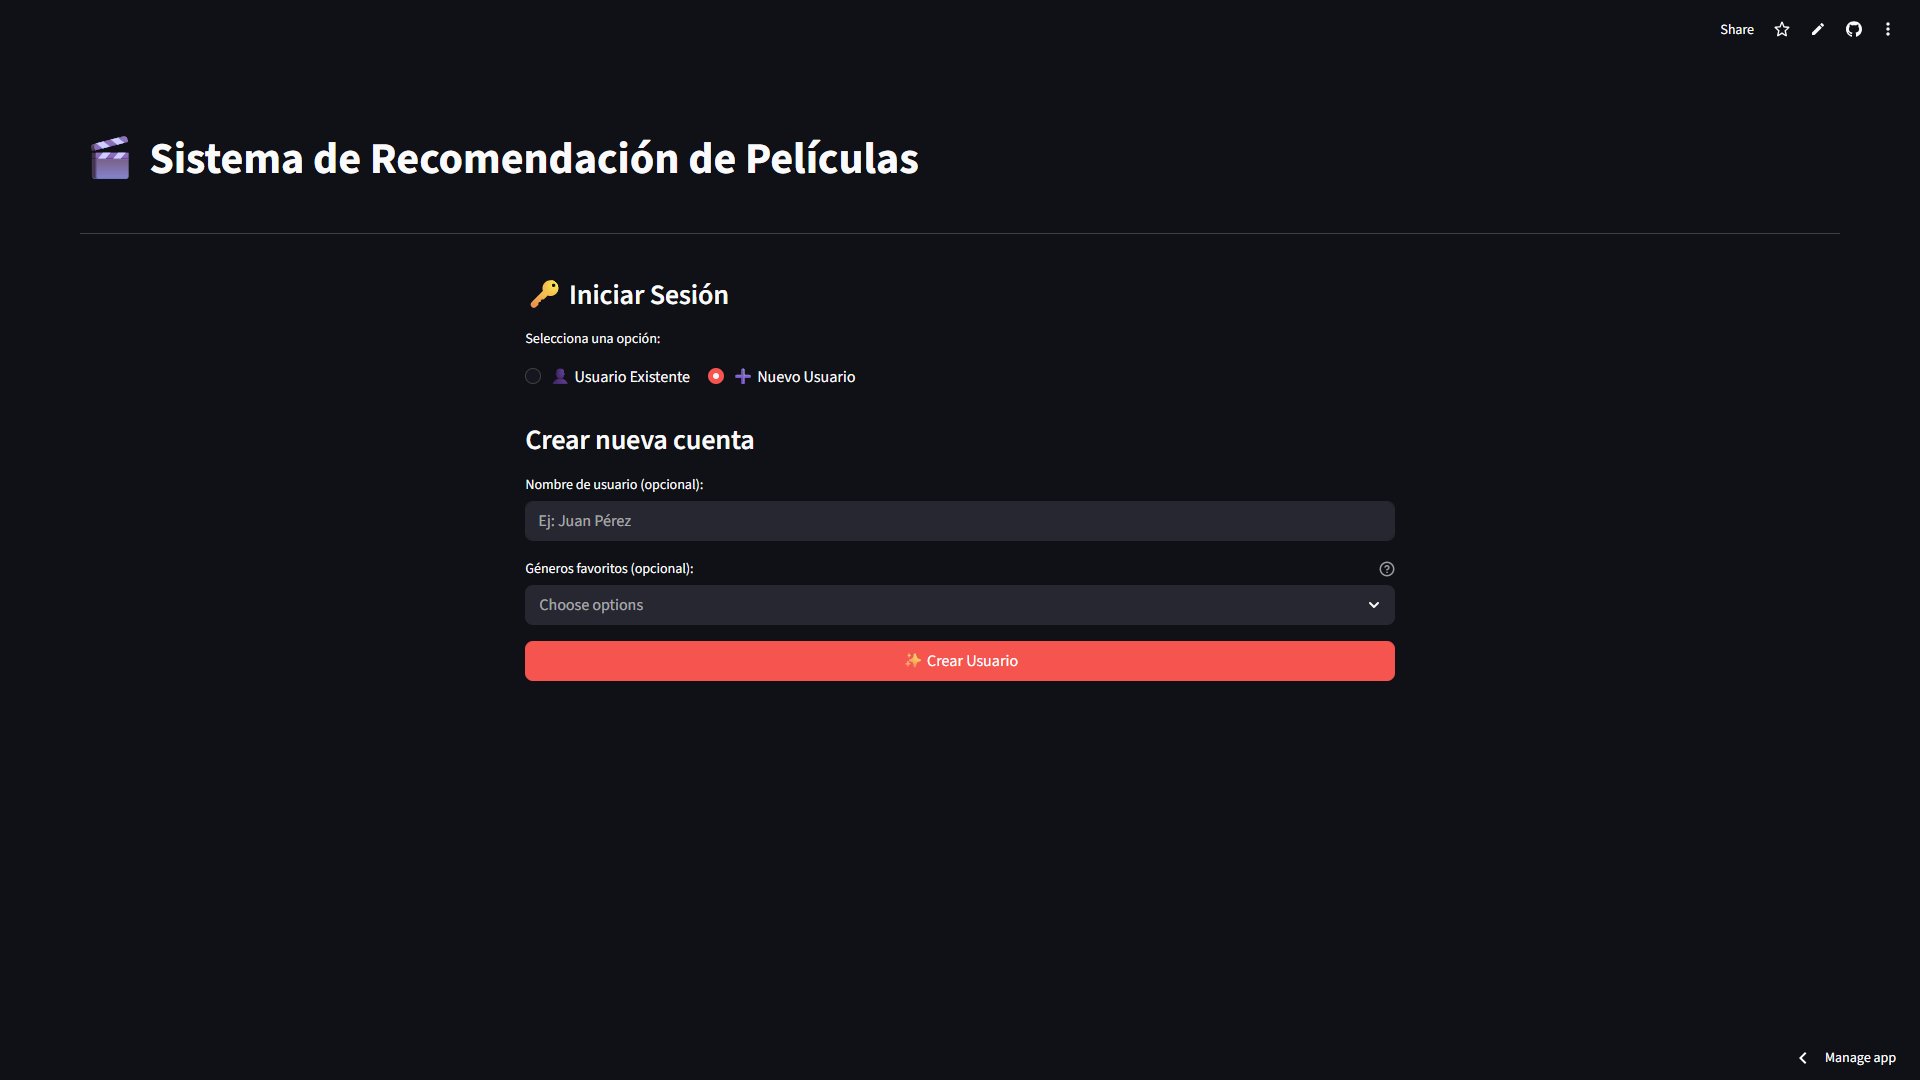
\includegraphics[width=0.82\textwidth]{new_user_window.png}
\caption{Creacion de un nuevo usuario y seleccion inicial de preferencias.}
\end{figure}

El usuario puede elegir la tecnica de recomendacion que desea aplicar. Esto permite comparar visualmente como cambia la lista de peliculas al pasar de contenido a colaborativo o hibrido para el mismo perfil.

\begin{figure}[htbp]
\centering
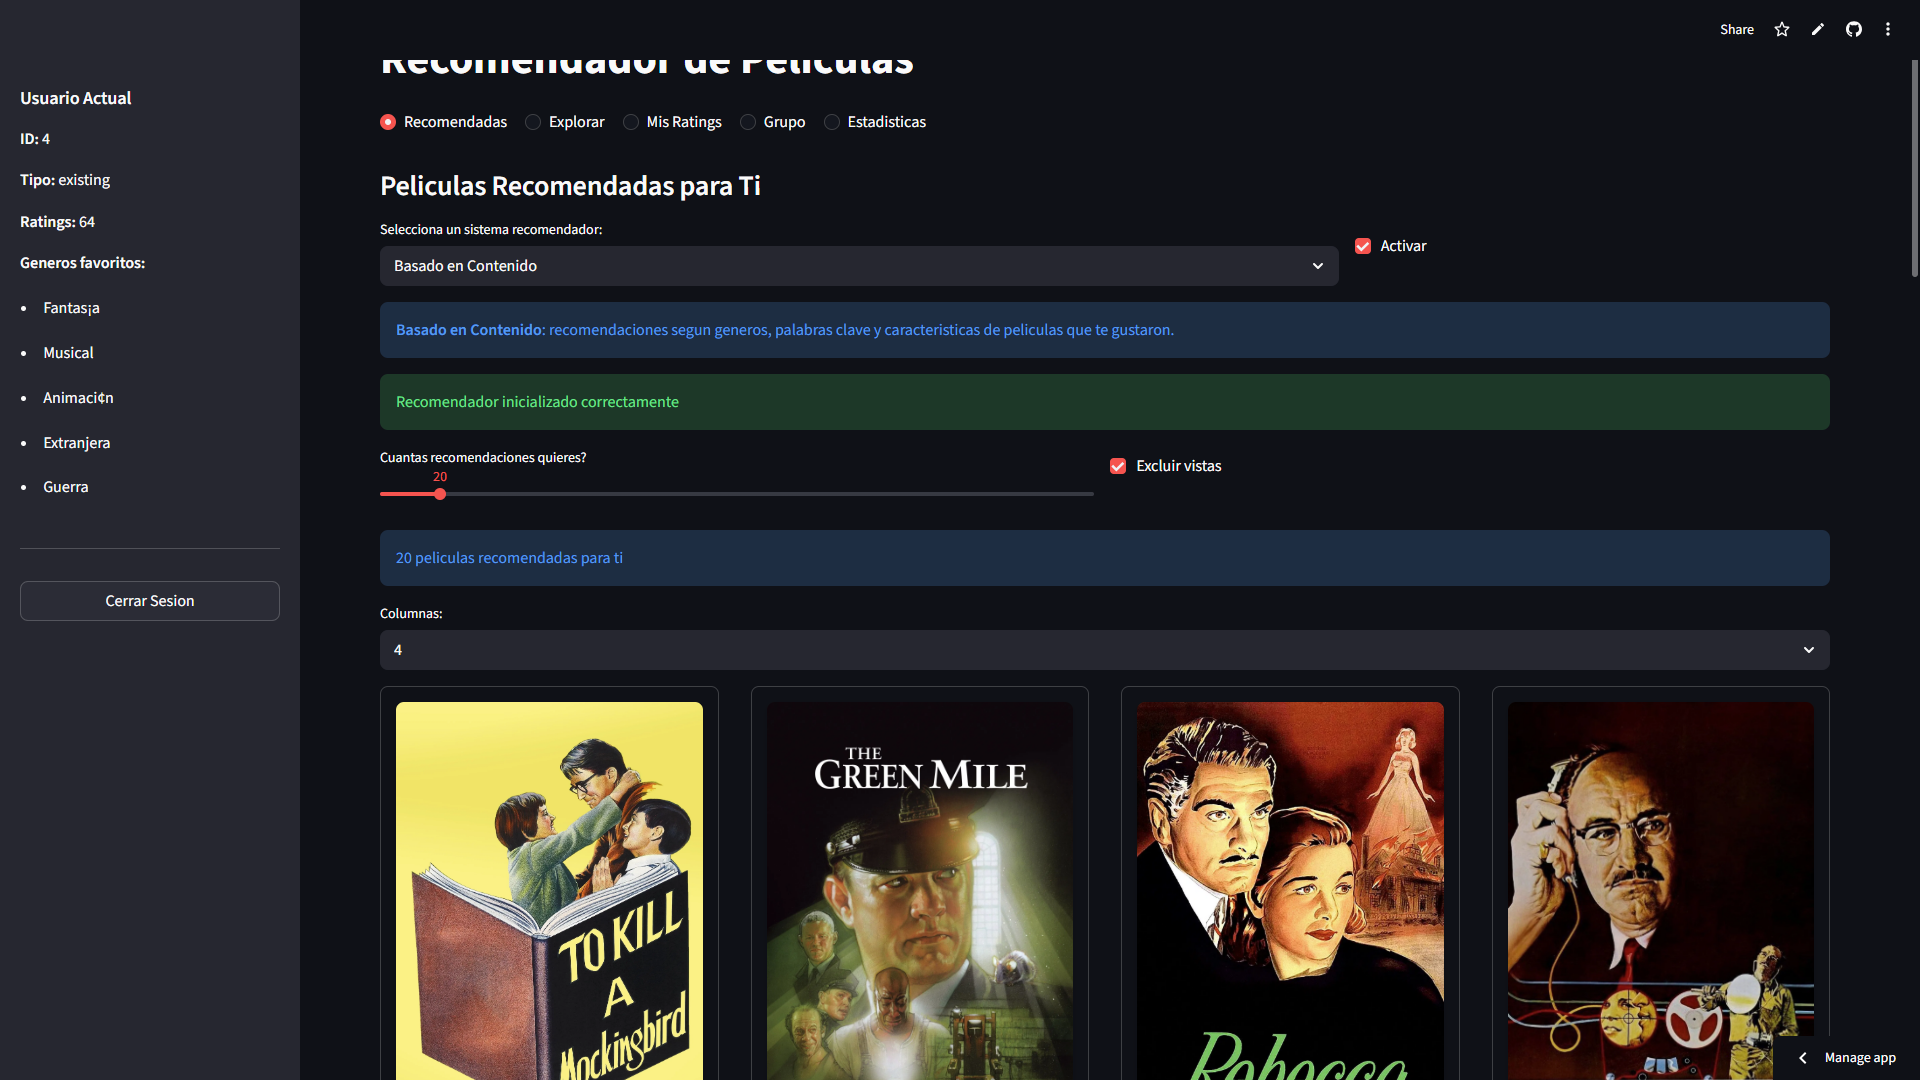
\includegraphics[width=0.95\textwidth]{Window_content_recomender.png}
\caption{Recomendaciones generadas por el sistema basado en contenido.}
\end{figure}

\begin{figure}[htbp]
\centering
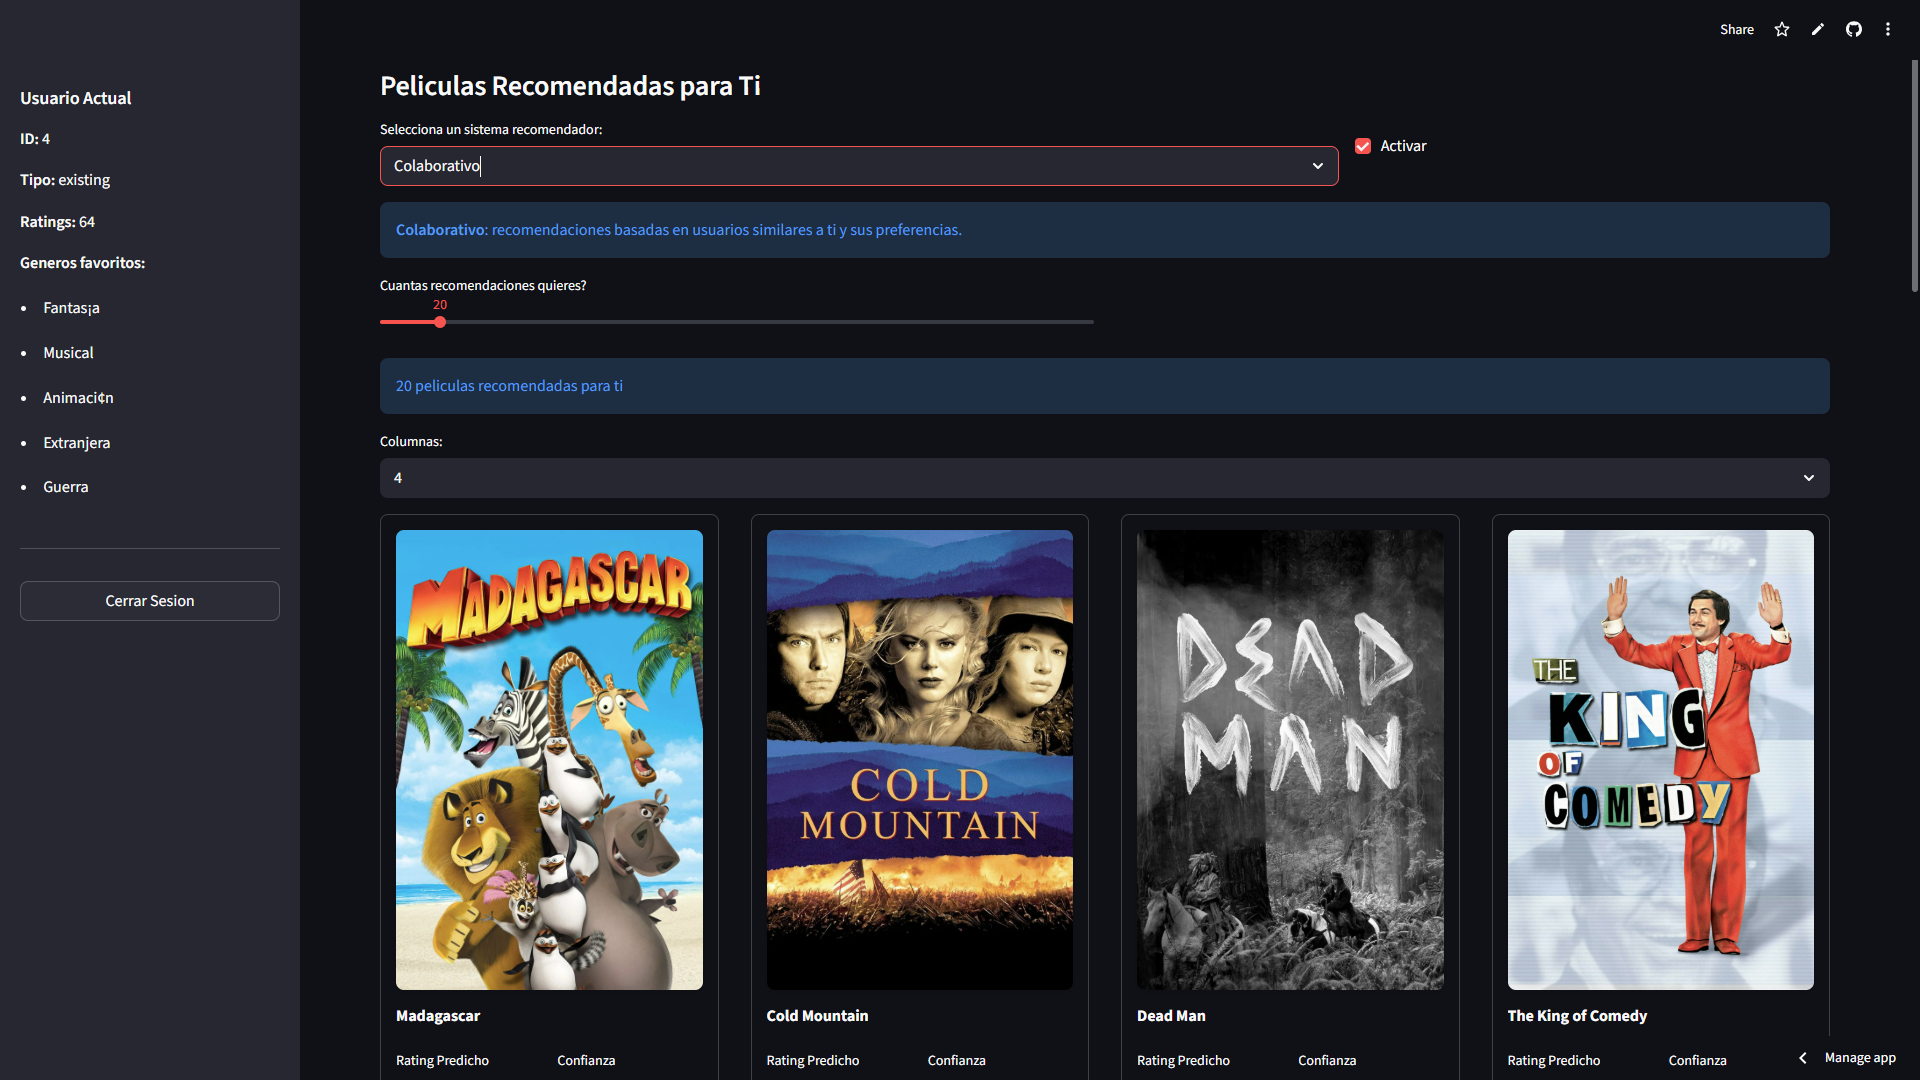
\includegraphics[width=0.95\textwidth]{window_colaborative_recomender.png}
\caption{Recomendaciones generadas por el sistema colaborativo.}
\end{figure}

\begin{figure}[htbp]
\centering
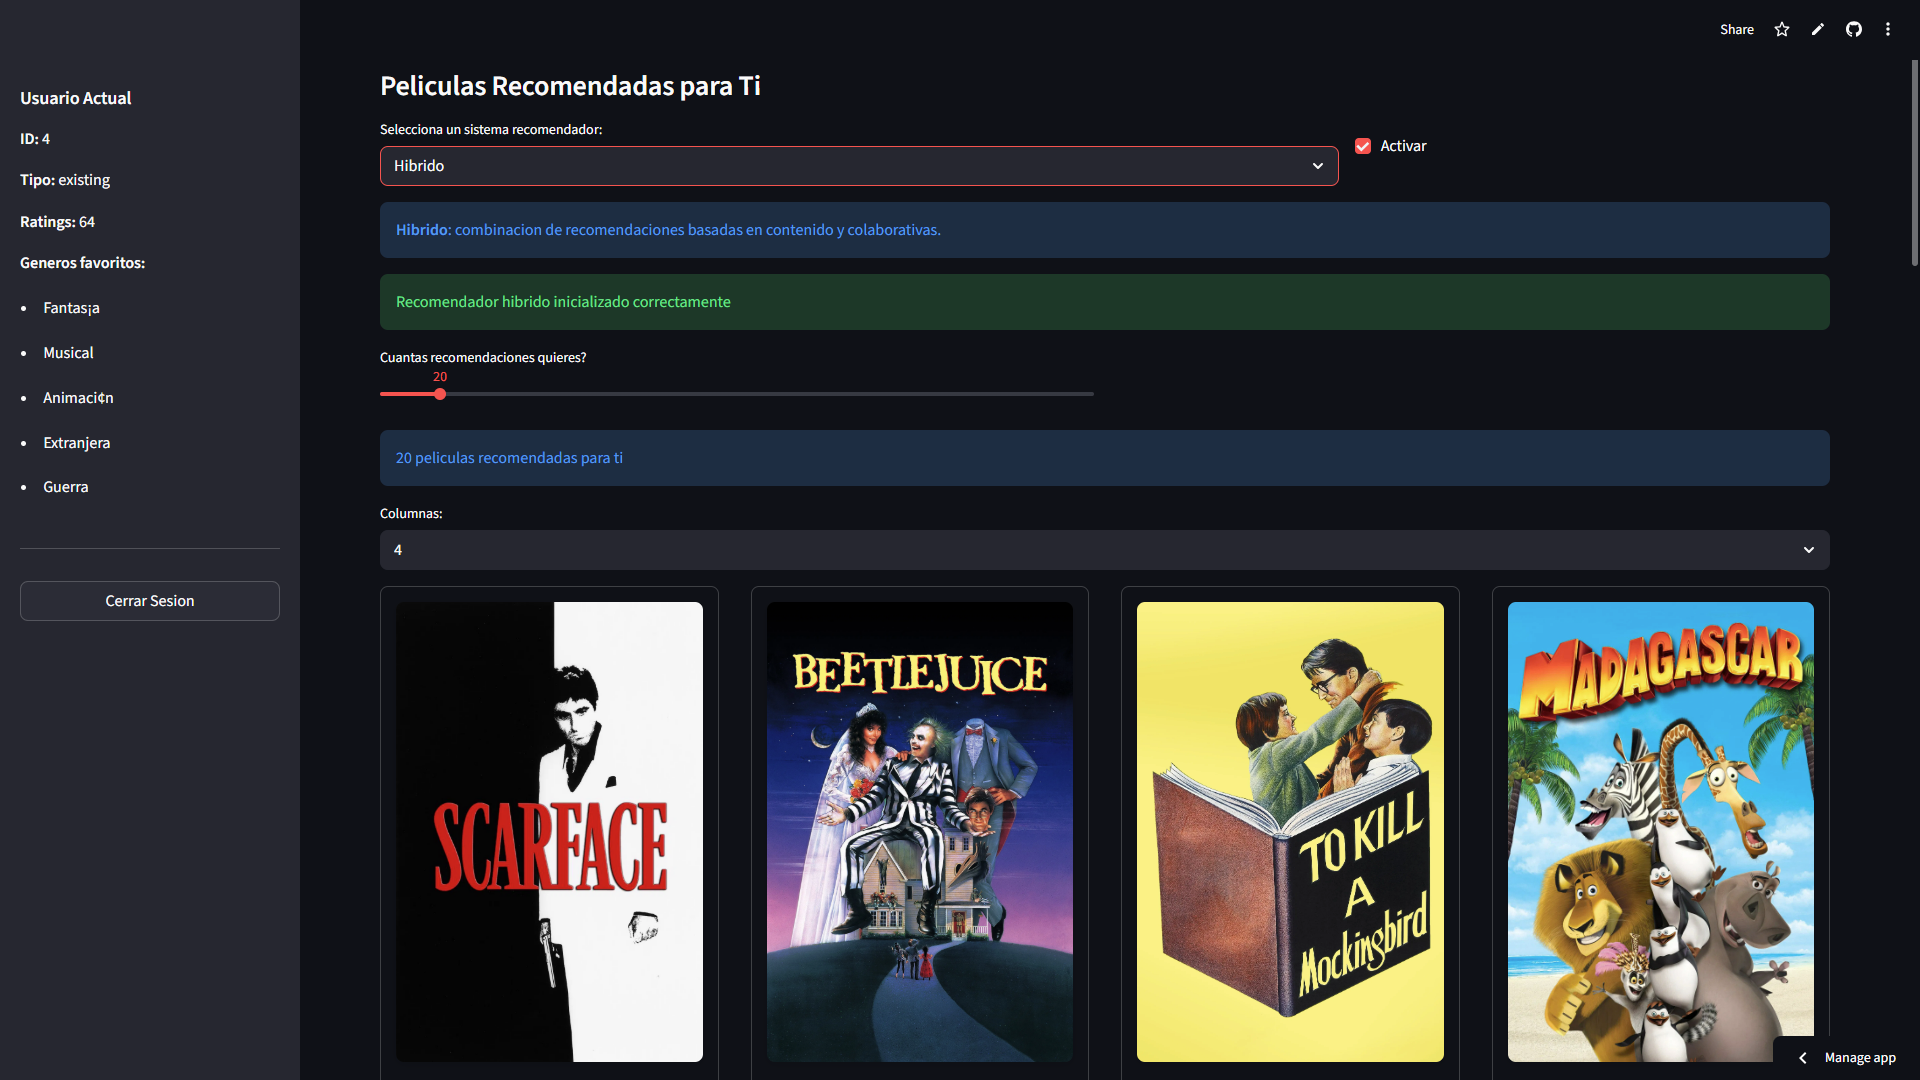
\includegraphics[width=0.95\textwidth]{Window_hybrid_recomender.png}
\caption{Recomendaciones generadas por el sistema hibrido.}
\end{figure}

Ademas, la aplicacion permite visualizar las valoraciones del usuario y estadisticas basicas de su perfil. Esto ayuda a entender por que cambian las recomendaciones entre usuarios: el sistema no recomienda sobre una sesion anonima, sino sobre un historial y un vector de preferencias persistente.

\begin{figure}[htbp]
\centering
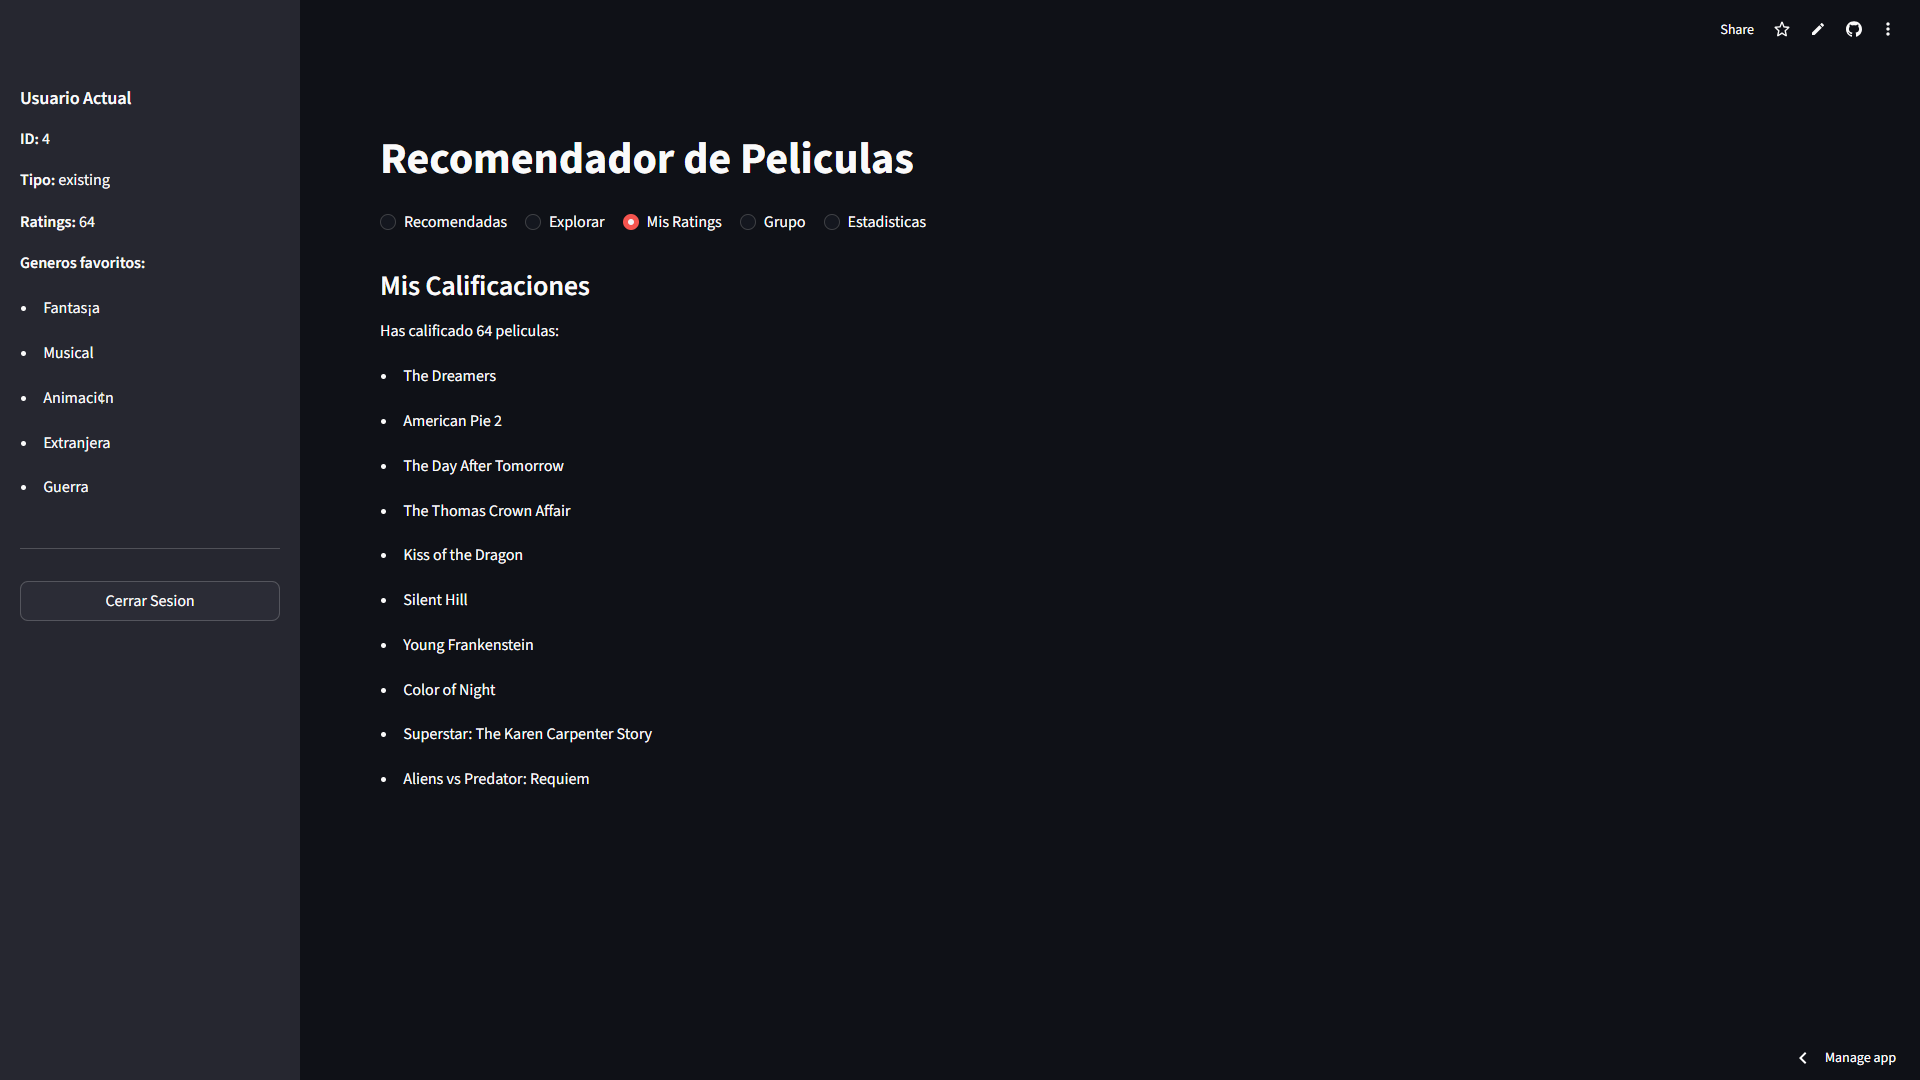
\includegraphics[width=0.82\textwidth]{Window_myratings.png}
\caption{Pantalla de valoraciones realizadas por el usuario.}
\end{figure}

\begin{figure}[htbp]
\centering
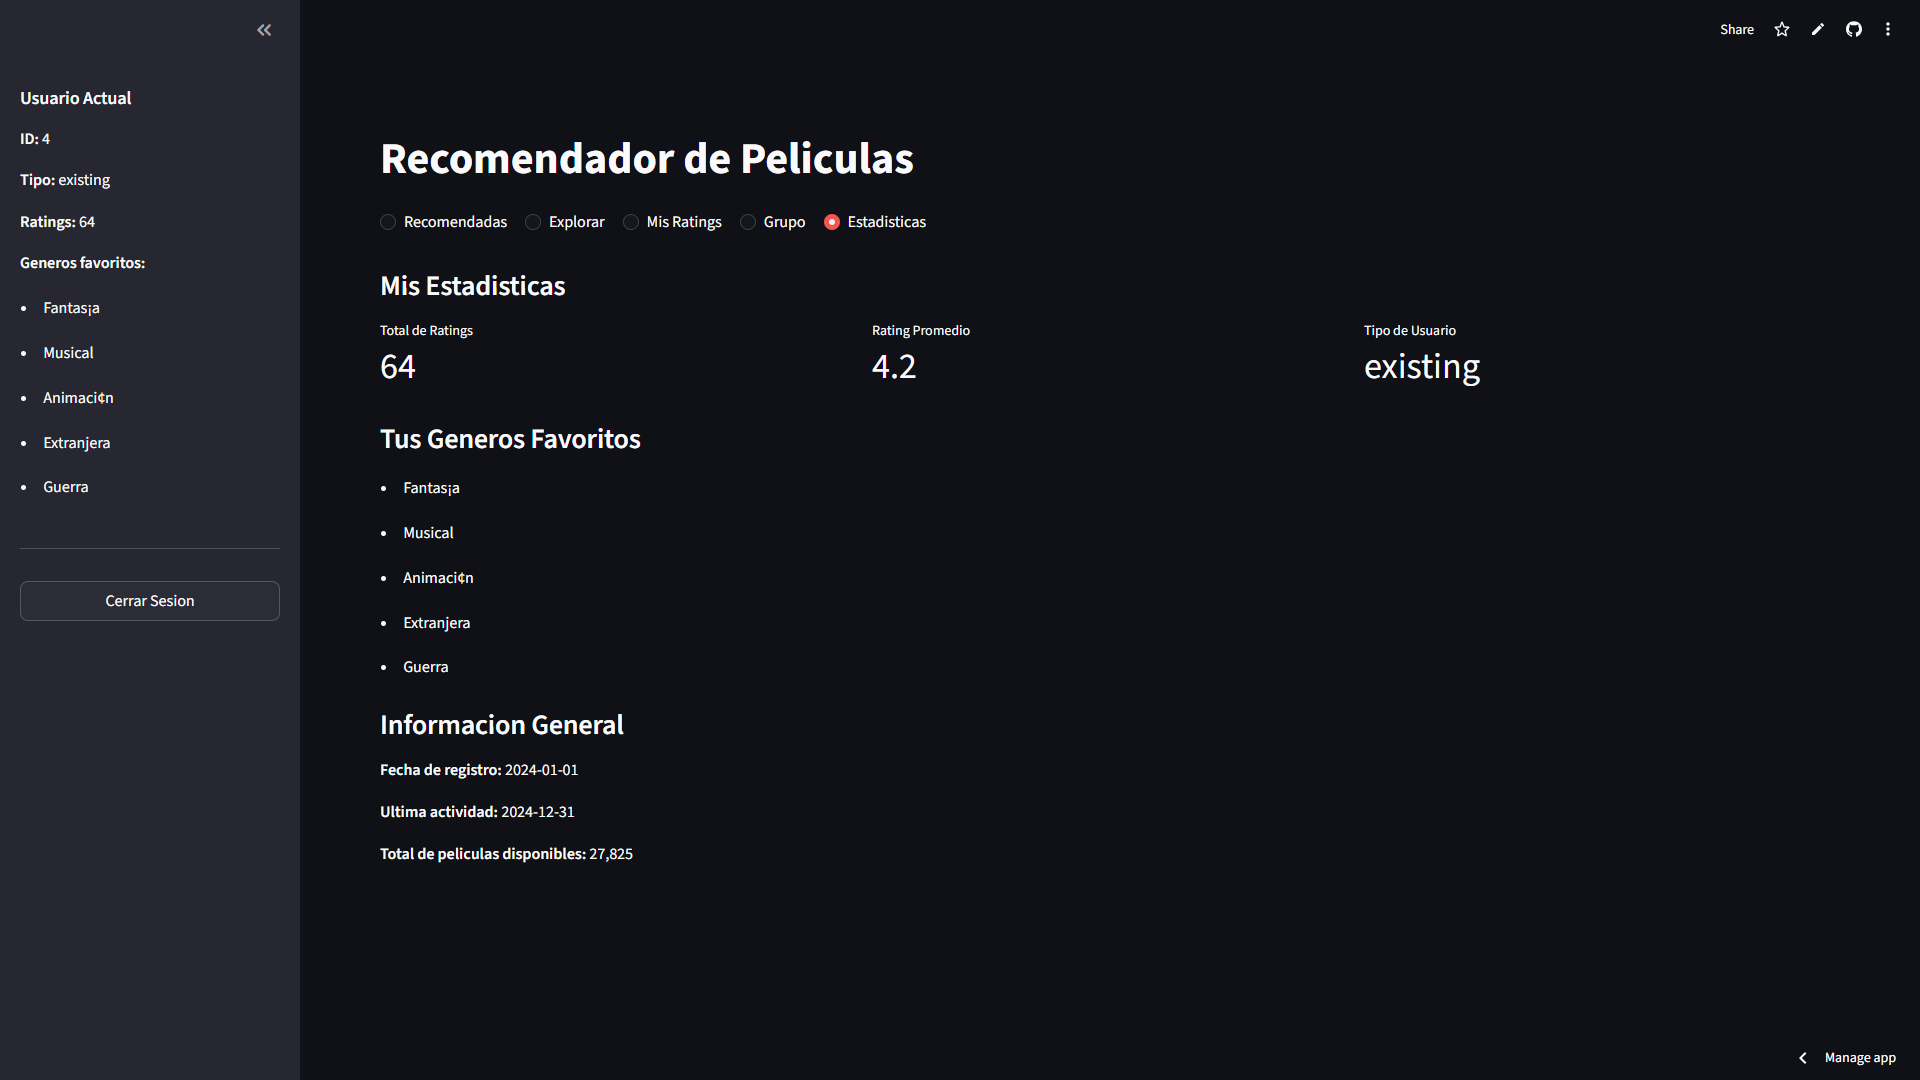
\includegraphics[width=0.82\textwidth]{window_stats.png}
\caption{Estadisticas del perfil del usuario.}
\end{figure}

La interfaz de grupo permite seleccionar usuarios registrados y obtener una recomendacion conjunta.

\begin{figure}[htbp]
\centering
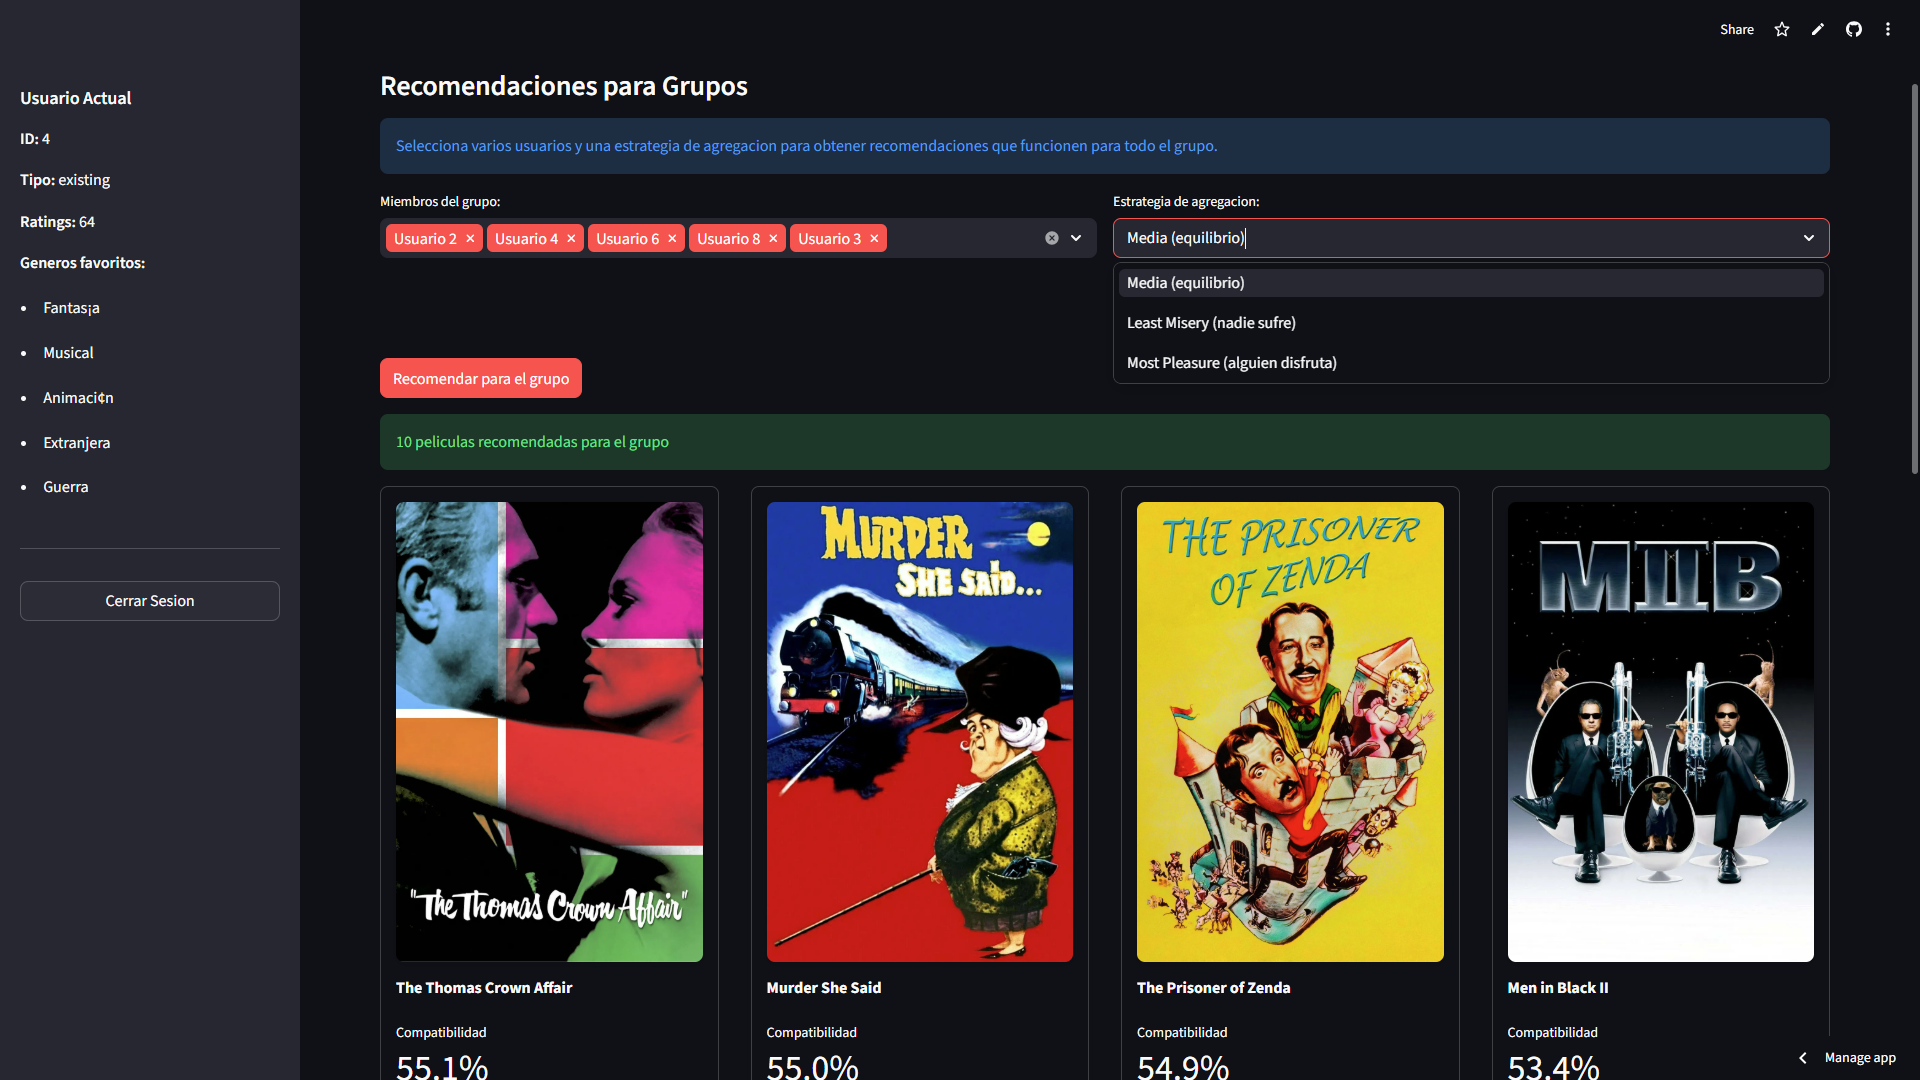
\includegraphics[width=0.95\textwidth]{Group_recomender.png}
\caption{Recomendador para grupos de usuarios registrados.}
\end{figure}

\section{Sistema recomendador basado en contenido}

\subsection{Idea general}

El recomendador basado en contenido compara el perfil del usuario con las caracteristicas de las peliculas. No necesita buscar usuarios similares; solo requiere una representacion de peliculas y una representacion del usuario en el mismo espacio.

Cada pelicula se representa mediante dos bloques principales: generos y texto. Los generos se codifican como etiquetas multiples, porque una pelicula puede pertenecer a varios generos. El texto se construye concatenando campos como \texttt{overview}, \texttt{tagline}, \texttt{keywords}, \texttt{tags}, reparto, equipo, director y generos normalizados. Ese documento se vectoriza con TF-IDF.

\subsection{Perfil del usuario}

El perfil del usuario combina dos senales:

\begin{itemize}[leftmargin=*]
\item \textbf{Perfil de generos}: procede del \texttt{genre\_vector} almacenado en el registro. Se reducen los generos menos informativos y se conservan aproximadamente los mas representativos.
\item \textbf{Perfil historico}: se obtiene agregando vectores de peliculas que el usuario ha valorado, ponderadas segun el rating.
\end{itemize}

La mezcla entre ambas partes permite que el sistema funcione con usuarios nuevos, pero que tambien se ajuste cuando el usuario va acumulando valoraciones reales.

\subsection{Calculo del ratio}

La puntuacion final de contenido para un usuario $u$ y una pelicula $i$ se calcula como una combinacion ponderada:

\[
r_{ui} =
\alpha \cdot Score_{contenido}(u,i) +
\beta \cdot Score_{calidad}(i) +
\gamma \cdot Score_{popularidad}(i) +
\delta \cdot Score_{similitud}(u,i)
\]

Los pesos utilizados son:

\[
\alpha = 0.50,\quad \beta = 0.20,\quad \gamma = 0.15,\quad \delta = 0.15
\]

El componente principal es la compatibilidad por contenido, pero se anaden senales de calidad, popularidad y similitud semantica. Esta decision evita recomendar peliculas muy ajustadas al perfil pero con informacion poco fiable o baja calidad general.

Cuando una pelicula pertenece a varios generos, el sistema calcula la afinidad con todos ellos y pondera el resultado para que las peliculas con muchas etiquetas no reciban ventaja artificial. Los items ya vistos se excluyen de la lista final.

\subsection{Decisiones destacadas}

\begin{itemize}[leftmargin=*]
\item Se usa TF-IDF porque permite representar texto de forma eficiente y da mas peso a terminos discriminativos.
\item Se reduce el vector de generos del usuario para evitar perfiles demasiado amplios y poco explicativos.
\item Se incorporan popularidad y calidad como senales secundarias, no como criterio dominante.
\item Las recomendaciones incluyen razones interpretables relacionadas con generos, similitud y calidad.
\end{itemize}

\section{Sistema recomendador colaborativo}

\subsection{Representacion de usuarios}

El recomendador colaborativo representa cada usuario mediante un vector de preferencias por genero:

\[
u = [pref_{accion}, pref_{comedia}, pref_{drama}, \ldots]
\]

La matriz usuario-genero contiene una fila por usuario activo y una columna por genero. En lugar de comparar directamente coincidencias exactas usuario-item, el sistema compara perfiles globales de gusto. Esta decision reduce la dispersion del dataset, ya que no todos los usuarios han puntuado las mismas peliculas.

\subsection{Obtencion de vecinos}

La afinidad entre usuarios se calcula con correlacion de Pearson:

\[
sim(u,v) =
\frac{\sum_k (p_{uk} - \bar{p_u})(p_{vk} - \bar{p_v})}
{\sqrt{\sum_k (p_{uk} - \bar{p_u})^2} \cdot \sqrt{\sum_k (p_{vk} - \bar{p_v})^2}}
\]

Solo se conservan vecinos con similitud positiva. Si dos usuarios tienen suficientes generos comunes con valor no nulo, la correlacion se calcula sobre esa interseccion. Si no hay solapamiento suficiente, se usa el vector completo. El umbral de solapamiento utilizado es:

\[
MIN\_COMMON\_PREFS = 10
\]

Finalmente se ordenan los vecinos por similitud y se conservan los mejores. La implementacion permite cachear la matriz de preferencias y guardar vecinos precalculados para acelerar el uso desde la interfaz.

\subsection{Generacion de candidatos}

Una pelicula candidata es una pelicula que cumple dos condiciones: ha sido valorada favorablemente por algun vecino y no aparece en el historial del usuario objetivo. Se considera valoracion favorable:

\[
rating \geq 3.5
\]

Si varios vecinos proponen la misma pelicula, el item no se duplica; se mantiene una unica entrada y despues se usa toda la evidencia disponible para predecir su rating.

\subsection{Prediccion del rating}

Para cada pelicula candidata se buscan los vecinos que la han puntuado. La prediccion se calcula como media ponderada por similitud:

\[
\hat{r}_{ui} =
\frac{\sum_{v \in V_u(i)} sim(u,v)\, r_{vi}}
{\sum_{v \in V_u(i)} |sim(u,v)|}
\]

Ademas del rating predicho, el sistema calcula una confianza basada en la similitud media y el numero de vecinos que contribuyen a la prediccion. El score de ranking se define como:

\[
ranking\_score(u,i) = \hat{r}_{ui} \cdot confidence(u,i)
\]

Esto evita que una pelicula con rating estimado alto pero apoyada por un unico vecino domine la lista final. Primero se priorizan recomendaciones con soporte suficiente y despues se ordenan por score, confianza y rating predicho.

\section{Sistema recomendador hibrido}

\subsection{Motivacion}

El recomendador hibrido combina las ventajas de los dos enfoques anteriores. El basado en contenido es robusto cuando hay un perfil individual claro, mientras que el colaborativo puede descubrir peliculas que no son evidentes por metadatos pero que han gustado a usuarios parecidos.

La recomendacion hibrida sigue tres pasos:

\begin{enumerate}[leftmargin=*]
\item Obtener una lista amplia de candidatos del recomendador basado en contenido.
\item Obtener una lista amplia de candidatos del recomendador colaborativo.
\item Unificar los items, normalizar sus scores y calcular un nuevo ratio hibrido.
\end{enumerate}

\subsection{Normalizacion y mezcla}

Los dos recomendadores no producen puntuaciones en la misma escala. El contenido devuelve un score aproximadamente en $[0,1]$, mientras que el colaborativo trabaja con ratings y confianza. Por tanto, antes de mezclar se normalizan ambas senales:

\[
r_{content}(i) = score_{content}(i)
\]

\[
r_{collab}(i) = \frac{ranking\_score(i)}{5}
\]

La mezcla final es:

\[
score_{hibrido}(u,i) =
\alpha_u \cdot r_{content}(u,i) +
\beta_u \cdot r_{collab}(u,i)
\]

con:

\[
\alpha_u + \beta_u = 1
\]

Los pesos no son fijos. Se calculan dinamicamente a partir de la informacion disponible para el usuario: calidad del perfil de contenido, historial, numero de candidatos, vecinos disponibles, similitud media y soporte colaborativo.

\subsection{Items repetidos}

Cuando una pelicula aparece en ambas listas, no se duplica. Se guarda una unica entrada y se suman las contribuciones normalizadas de contenido y colaborativo. Si solo aparece en una de las listas, la contribucion ausente vale cero. En el ranking final se ordena por score hibrido y, en caso de empate, se favorecen items que aparecen en ambos recomendadores.

Esta estrategia hace que el hibrido pueda actuar de dos formas: reforzar peliculas en las que ambos modelos coinciden o recuperar peliculas buenas de una sola fuente cuando la otra no tiene suficiente evidencia.

\section{Sistema recomendador para grupos}

El recomendador para grupos permite seleccionar varios usuarios registrados y generar una lista comun. La decision de tamano maximo del grupo se deja abierta en la aplicacion: no se fija un limite algoritmico estricto, mas alla de la usabilidad de la interfaz y del coste de calcular recomendaciones individuales para todos los miembros seleccionados.

La rubrica permite usar la tecnica de recomendacion que se quiera siempre que sea la misma para todos los miembros del grupo. En la version implementada, el recomendador de grupo utiliza el recomendador colaborativo como tecnica base. Esta eleccion es coherente con el objetivo del modo grupo porque el colaborativo ya produce un \texttt{ranking\_score} que combina rating predicho, similitud con vecinos y confianza. Sobre esa puntuacion individual se aplica despues la agregacion grupal.

El proceso es:

\begin{enumerate}[leftmargin=*]
\item Seleccionar los usuarios del grupo.
\item Seleccionar una misma tecnica base para todos los miembros. En la implementacion actual se usa la colaborativa.
\item Obtener recomendaciones individuales para cada miembro.
\item Eliminar cualquier pelicula que este en el historico de alguno de los usuarios del grupo.
\item Crear el conjunto union de peliculas candidatas.
\item Asignar a cada pelicula los scores individuales de cada usuario.
\item Agregar esos scores con la estrategia seleccionada para obtener el ratio de interes del grupo.
\item Ordenar por score grupal y devolver el top final.
\end{enumerate}

Formalmente, para una pelicula $i$ y un grupo $G$, primero se obtiene el score individual $r_{u,i}$ de cada usuario $u$. Si el item no aparece en la lista recomendada de un usuario, se asigna:

\[
r_{u,i}=0
\]

De esta forma, el ratio grupal depende de dos factores pedidos en la rubrica: el valor que recibe el item en las listas individuales y el numero de usuarios para los que aparece recomendado. Un item recomendado por varios miembros acumula mas evidencia que un item que solo aparece para una persona.

Se contemplan tres estrategias de agregacion:

\begin{itemize}[leftmargin=*]
\item \textbf{Average}: calcula la media de los scores individuales:
\[
score_G(i)=\frac{1}{|G|}\sum_{u \in G} r_{u,i}
\]
Prioriza consenso general. Si un item aparece para varios usuarios con puntuaciones altas, sube en el ranking; si solo aparece para uno, queda penalizado por los ceros del resto.
\item \textbf{Least misery}: calcula el minimo:
\[
score_G(i)=\min_{u \in G} r_{u,i}
\]
Es una estrategia conservadora. Evita recomendar peliculas que puedan ser malas para algun miembro, pero tambien puede ser muy restrictiva porque una ausencia en una lista individual equivale a 0.
\item \textbf{Most pleasure}: calcula el maximo:
\[
score_G(i)=\max_{u \in G} r_{u,i}
\]
Favorece peliculas que gusten mucho al menos a una persona. Es util cuando el objetivo es encontrar opciones fuertes para algun miembro, aunque ofrece menos garantia de consenso.
\end{itemize}

La estrategia principal que se propone para un uso general es \textbf{Average}, porque es la mas interpretable y equilibra las preferencias de todos los usuarios. Tambien responde bien a la pregunta de si es mejor que un item aparezca en mas de una lista: con media y ceros para ausentes, un item apoyado por varios usuarios queda naturalmente favorecido frente a otro que solo convence a uno. \emph{Least misery} y \emph{most pleasure} se mantienen como alternativas para escenarios distintos: evitar rechazo individual o maximizar satisfaccion de algun miembro.

La lista final no contiene items repetidos. Si una pelicula aparece en varias listas individuales, se mantiene una unica entrada y se combinan sus ratios. Si una pelicula aparece en el historico de cualquier miembro del grupo, se elimina antes de calcular el ranking final. La interfaz muestra finalmente las peliculas ordenadas por el ratio grupal calculado.

\section{Evaluacion}

\subsection{Protocolo}

La evaluacion offline se realiza solo con usuarios del dataset. Se seleccionan 20 usuarios aleatoriamente con semilla fija, y los mismos usuarios se usan para todas las metricas y todos los recomendadores. Para cada usuario se generan 50 recomendaciones con cada tecnica: contenido, colaborativo e hibrido.

Antes de evaluar, el conjunto de test se filtra para eliminar peliculas que ya no existen en el catalogo procesado. Esto sigue la indicacion del enunciado y evita comparar contra items imposibles de recomendar.

Los usuarios evaluados son:

\[
81, 96, 122, 188, 201, 205, 270, 288, 363, 383, 384, 385, 400, 420, 442, 481, 524, 610, 612, 620
\]

\subsection{Metricas}

Para precision, recall, F1 y nDCG se usan listas de items relevantes. Un item recomendado se considera relevante si su puntuacion recomendada supera el umbral:

\[
UMBRAL\_REC = 3.5
\]

Un item de test se considera relevante si su rating real supera:

\[
UMBRAL\_TEST = 3.5
\]

La precision mide que proporcion de los items recomendados como relevantes aparece tambien como relevante en test:

\[
Precision = \frac{Recomendados \cap Relevantes}{Recomendados}
\]

El recall mide que proporcion de los items relevantes de test han sido recuperados:

\[
Recall = \frac{Recomendados \cap Relevantes}{Relevantes}
\]

El F1 combina precision y recall:

\[
F1 = 2 \cdot \frac{Precision \cdot Recall}{Precision + Recall}
\]

El MAE compara ratings predichos y reales usando solo la interseccion entre recomendaciones y peliculas puntuadas en test:

\[
MAE = \frac{1}{N}\sum_{i=1}^{N} |p_i-r_i|
\]

El nDCG evalua la calidad del orden. Para cada recomendacion, si el item aparece en test relevante recibe como score su rating de test; si no aparece, recibe 0. El resultado se normaliza contra el ranking ideal del test:

\[
nDCG = \frac{DCG_{rec}}{IDCG_{test}}
\]

\subsection{Promedios obtenidos}

\begin{table}[htbp]
\centering
\caption{Promedio de metricas por recomendador.}
\begin{tabular}{lrrrrr}
\toprule
SR & Precision & Recall & F1 & MAE & nDCG \\
\midrule
BC & 0.0410 & 0.2922 & 0.0662 & 0.8337 & 0.1406 \\
Col & 0.0422 & 0.2419 & 0.0663 & 0.7699 & 0.1251 \\
Hibrido & 0.0849 & 0.1043 & 0.0616 & 0.9872 & 0.0639 \\
\bottomrule
\end{tabular}
\end{table}

Los valores de precision son bajos en general. Esto es esperable porque se recomiendan 50 peliculas por usuario, pero el conjunto de test de cada usuario es pequeno. Muchos usuarios tienen entre 5 y 16 ratings en test, por lo que la probabilidad de que una recomendacion coincida exactamente con una pelicula oculta del test es reducida. La evaluacion es estricta: una recomendacion puede ser razonable para el perfil del usuario, pero si el usuario no la puntuo en test cuenta como fallo para precision, recall y nDCG.

\subsection{Precision, recall y F1 por recomendador}

\begin{figure}[htbp]
\centering
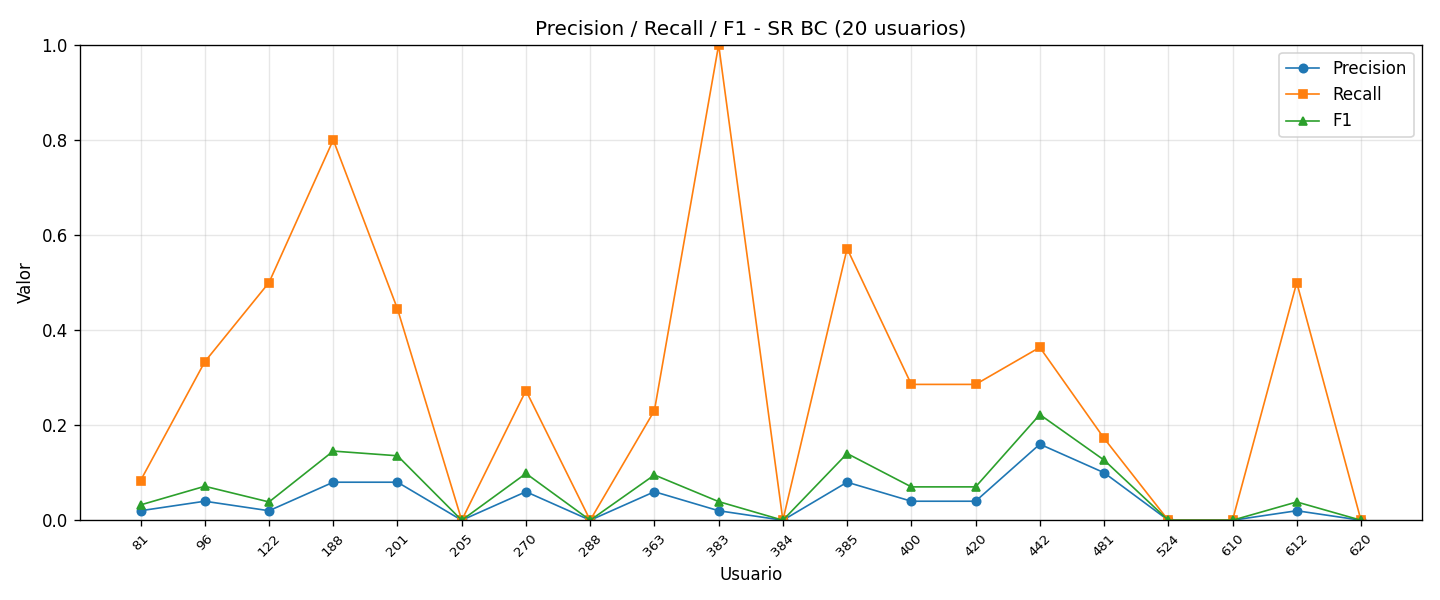
\includegraphics[width=0.95\textwidth]{01_PRF1_BC.png}
\caption{Precision, recall y F1 del recomendador basado en contenido.}
\end{figure}

El recomendador basado en contenido muestra precision baja pero recall relativamente alto en varios usuarios. Esto indica que genera listas amplias que capturan parte de las peliculas relevantes de test, aunque tambien marca como relevantes muchas peliculas que no aparecen en el conjunto de prueba. El caso mas claro es el usuario 383, donde el recall llega a 1.0, pero la precision se mantiene en 0.02. Esto significa que recupera todos los items relevantes disponibles en test, pero dentro de una lista con muchos candidatos.

\begin{figure}[htbp]
\centering
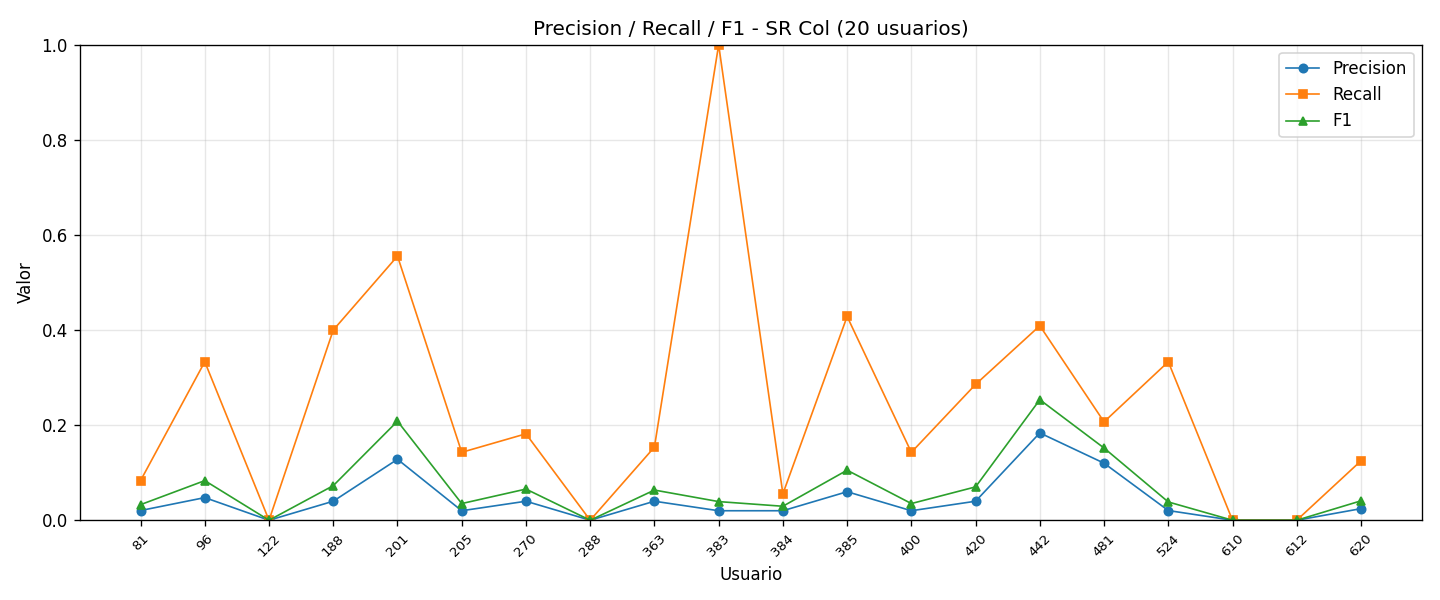
\includegraphics[width=0.95\textwidth]{01_PRF1_Col.png}
\caption{Precision, recall y F1 del recomendador colaborativo.}
\end{figure}

El colaborativo tiene un comportamiento parecido al contenido en F1 medio, pero con un MAE mejor. Su precision media es ligeramente superior a la de contenido, y su recall medio algo menor. Esto sugiere que el colaborativo predice mejor las notas cuando existe interseccion con test, pero no siempre coloca suficientes peliculas relevantes dentro de la lista recomendada. La razon principal es que depende de vecinos y de solapamiento: si los vecinos no han puntuado peliculas que tambien aparecen en el test del usuario objetivo, la metrica de acierto por item queda limitada.

\begin{figure}[htbp]
\centering
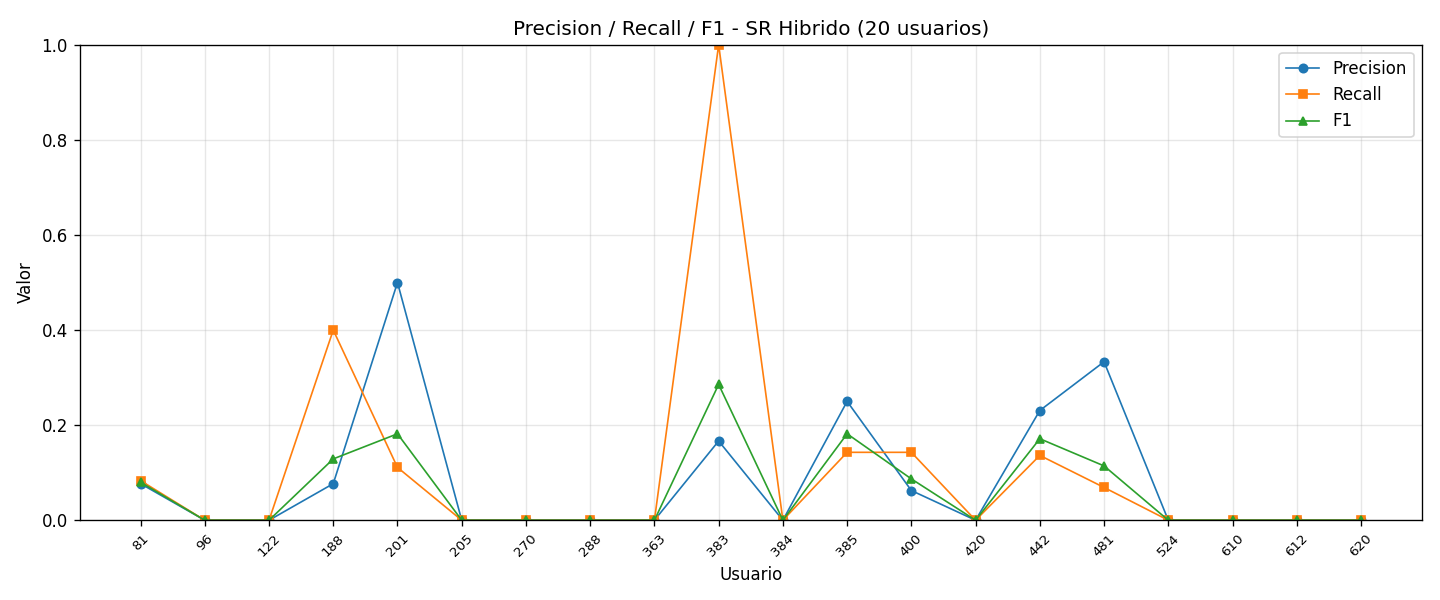
\includegraphics[width=0.95\textwidth]{01_PRF1_Hibrido.png}
\caption{Precision, recall y F1 del recomendador hibrido.}
\end{figure}

El hibrido obtiene la mejor precision media, 0.0849, pero el recall mas bajo, 0.1043. Esto indica que tiende a ser mas selectivo: cuando recomienda algo relevante, la proporcion de aciertos dentro de sus relevantes es mayor, pero cubre menos items relevantes del test. En usuarios como 201, 383, 385, 442 y 481 alcanza precision alta respecto a los otros modelos. Sin embargo, en muchos usuarios devuelve cero en recall y nDCG, lo que reduce mucho su media global.

\subsection{Comparacion entre tecnicas}

\begin{figure}[htbp]
\centering
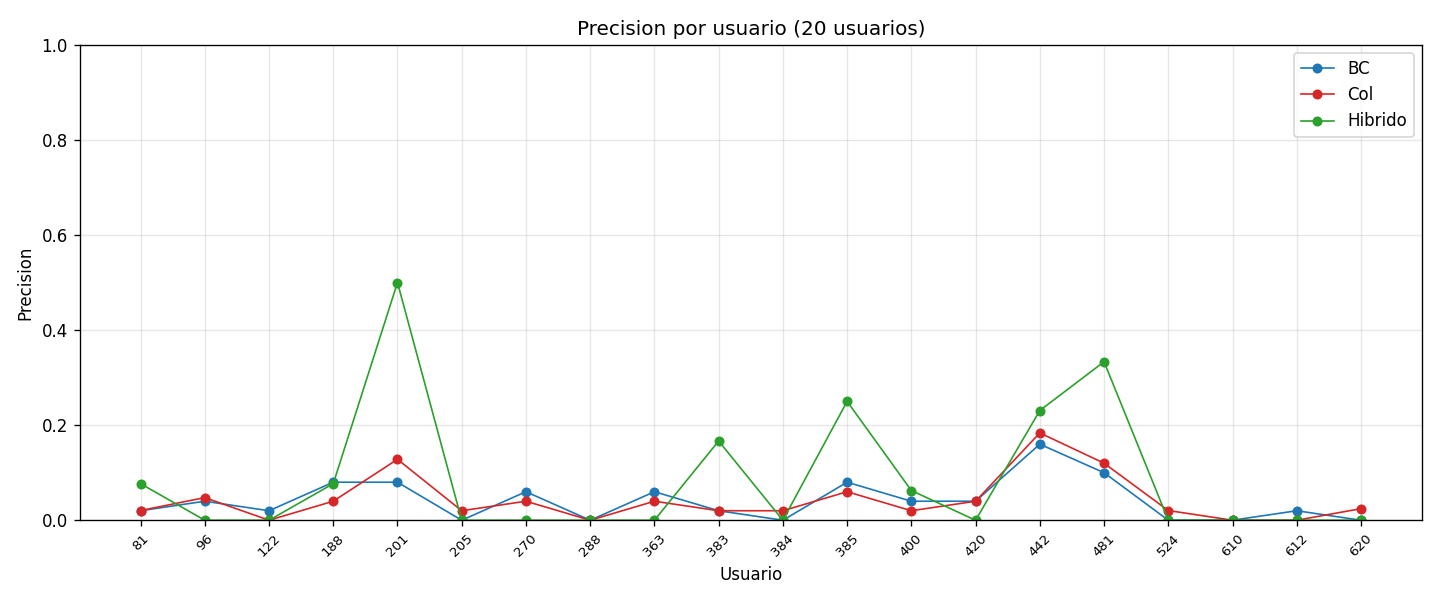
\includegraphics[width=0.95\textwidth]{02_Precision_comparativa.png}
\caption{Comparacion de precision entre recomendadores.}
\end{figure}

La precision favorece al hibrido. El motivo es que la mezcla de contenido y colaborativo filtra mejor los items cuando ambas senales aportan informacion. Sin embargo, esta mejora de precision viene acompanada de perdida de cobertura. El hibrido no necesariamente recupera muchos items relevantes de test, sino que reduce el conjunto de recomendaciones consideradas relevantes por encima del umbral.

\begin{figure}[htbp]
\centering
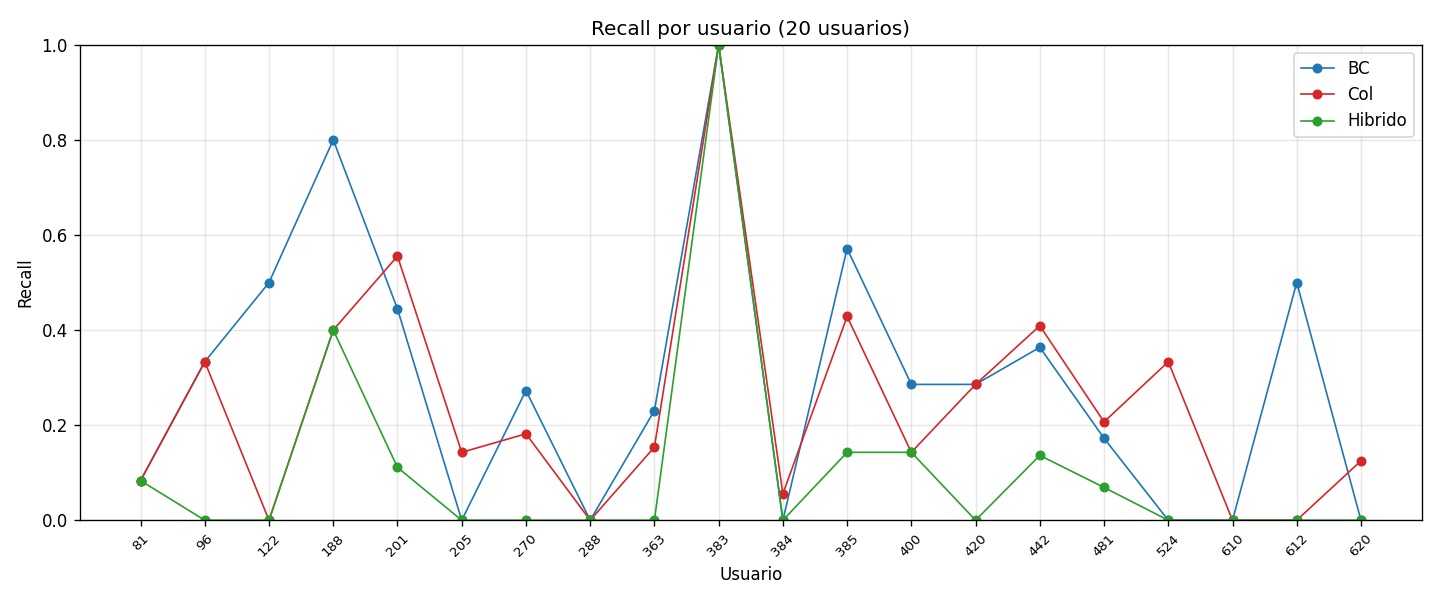
\includegraphics[width=0.95\textwidth]{03_Recall_comparativa.png}
\caption{Comparacion de recall entre recomendadores.}
\end{figure}

El recall favorece al basado en contenido y al colaborativo. El contenido alcanza el mejor promedio de recall, 0.2922, porque genera recomendaciones muy alineadas con generos y texto del perfil, de modo que tiene mas probabilidad de cubrir algun item relevante del test. El colaborativo queda cerca, con 0.2419. El hibrido baja a 0.1043 porque su ranking combinado es mas restrictivo y puede desplazar items que estaban en una lista base pero no reciben suficiente apoyo conjunto.

\begin{figure}[htbp]
\centering
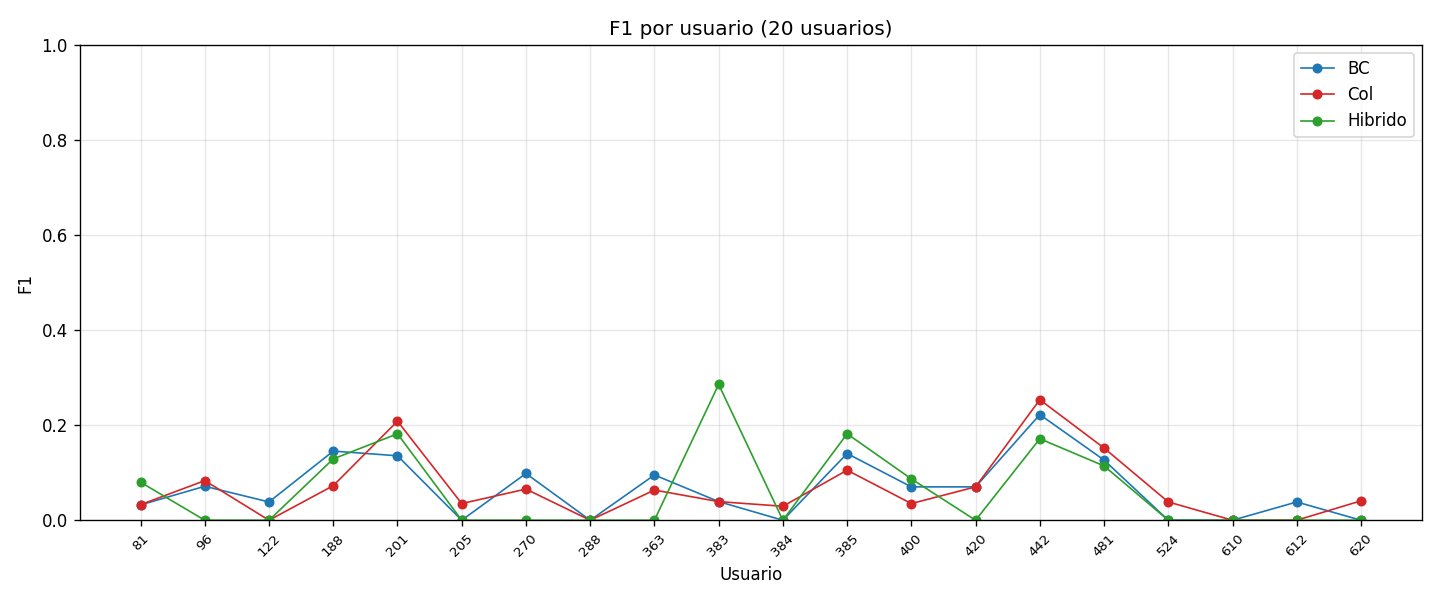
\includegraphics[width=0.95\textwidth]{04_F1_comparativa.png}
\caption{Comparacion de F1 entre recomendadores.}
\end{figure}

El F1 medio queda practicamente empatado entre contenido y colaborativo: 0.0662 frente a 0.0663. El hibrido baja ligeramente a 0.0616. Esta metrica muestra el compromiso entre precision y recall: aunque el hibrido mejora precision, pierde demasiado recall para superar a los otros modelos en media. En cambio, para usuarios concretos como 383, el hibrido obtiene el mejor F1 individual, 0.2857, porque combina una precision razonable con recall perfecto.

\subsection{MAE}

\begin{figure}[htbp]
\centering
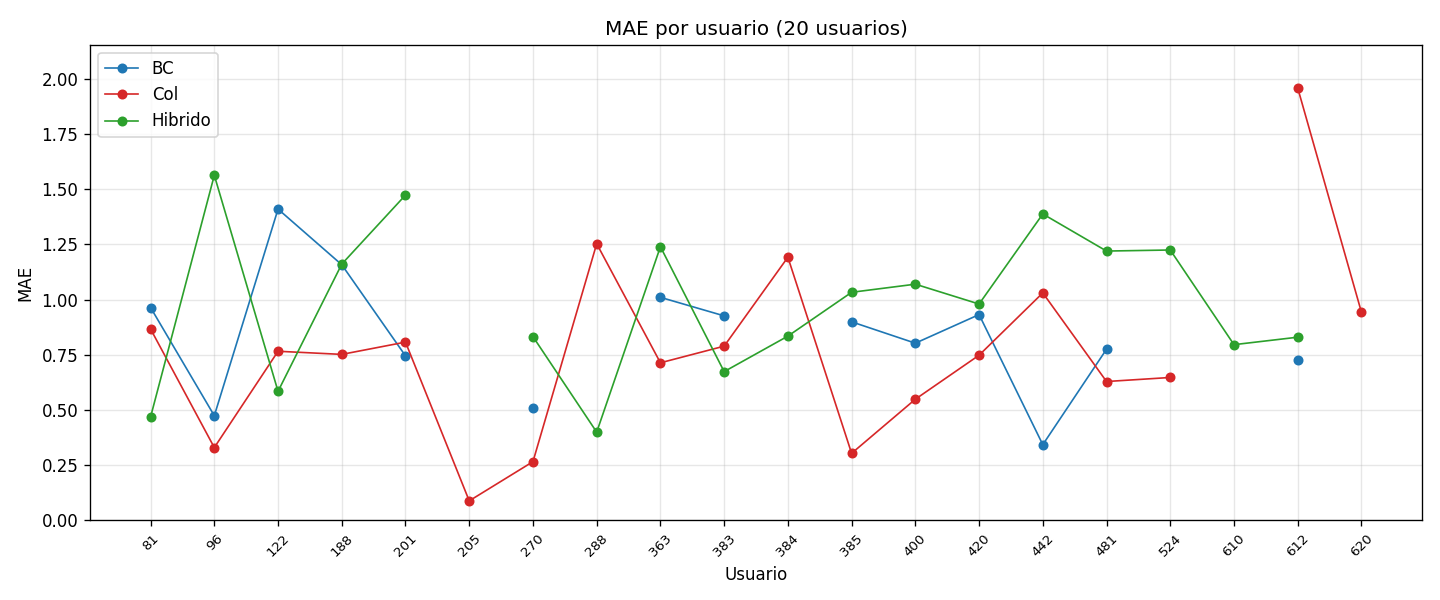
\includegraphics[width=0.95\textwidth]{05_MAE_comparativa.png}
\caption{Comparacion de MAE entre recomendadores.}
\end{figure}

El MAE mide la diferencia entre rating predicho y rating real en la interseccion entre recomendados y test. El mejor promedio lo obtiene el colaborativo, con 0.7699. Esto es coherente con su diseno: es el unico modelo que predice ratings directamente a partir de ratings de vecinos. El contenido y el hibrido convierten scores normalizados a escala de rating para poder calcular MAE, por lo que sus valores son menos naturales como prediccion numerica.

Tambien se observa que en algunos usuarios el MAE de contenido aparece vacio. Esto ocurre cuando no hay interseccion entre las peliculas recomendadas y las peliculas puntuadas por el usuario en test. En esos casos no existe una comparacion valida de rating y el script no fuerza un valor artificial.

El mejor caso individual de MAE es el usuario 205 con el colaborativo, con 0.0879. Esto indica que, para ese usuario y esa interseccion, los vecinos aportaron una prediccion muy cercana a las puntuaciones reales.

\subsection{nDCG}

\begin{figure}[htbp]
\centering
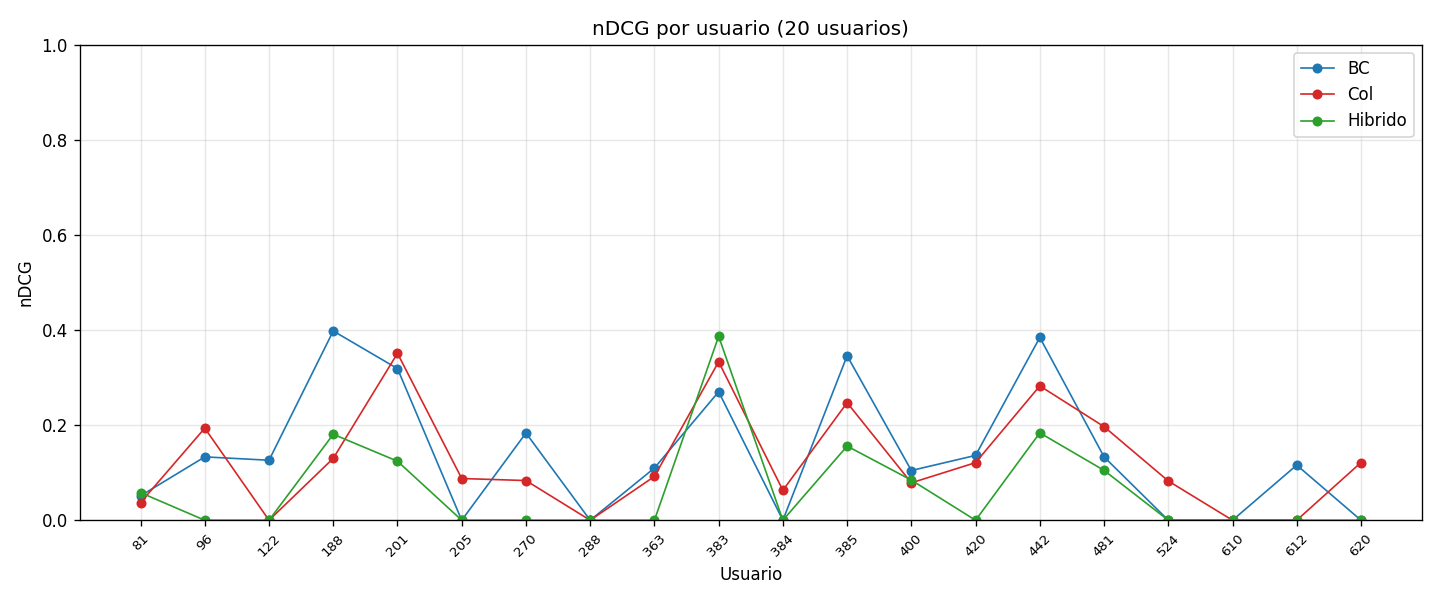
\includegraphics[width=0.95\textwidth]{06_nDCG_comparativa.png}
\caption{Comparacion de nDCG entre recomendadores.}
\end{figure}

El nDCG favorece al basado en contenido, con 0.1406 de media, seguido del colaborativo con 0.1251. El hibrido queda por debajo, con 0.0639. Esto significa que, cuando el contenido acierta items relevantes, suele situarlos en posiciones relativamente mejores dentro de la lista recomendada. El mejor nDCG individual es el del usuario 188 con contenido, 0.3981.

El resultado del hibrido en nDCG es especialmente interesante. Aunque mejora la precision media, no ordena tan bien respecto al ranking ideal del test. Esto puede explicarse porque el hibrido combina dos listas amplias y premia el acuerdo o la fuerza conjunta de las senales, pero el orden ideal de test depende solo de las valoraciones reales ocultas. Si un item relevante aparece en una fuente pero no en la otra, puede quedar desplazado por items con mejor score hibrido pero que no aparecen en test.

\subsection{Interpretacion global}

Los resultados muestran tres comportamientos distintos:

\begin{itemize}[leftmargin=*]
\item \textbf{Contenido}: mejor recall y mejor nDCG medio. Es el modelo que mejor cubre items relevantes y los ordena de forma mas cercana al ideal, pero su precision es baja porque genera muchas recomendaciones relevantes segun perfil que no aparecen en test.
\item \textbf{Colaborativo}: mejor MAE y F1 medio practicamente empatado con contenido. Es el mas fiable para estimar ratings cuando hay interseccion, pero depende de que existan vecinos utiles y ratings compartidos.
\item \textbf{Hibrido}: mejor precision media. Es mas selectivo y puede acertar mejor en usuarios concretos, pero pierde recall y nDCG porque algunos items relevantes de las listas base quedan desplazados por la mezcla.
\end{itemize}

Por tanto, no hay un ganador absoluto para todas las metricas. Si se prioriza recuperar el mayor numero de peliculas relevantes, el contenido es preferible. Si se prioriza aproximar la nota que daria el usuario, el colaborativo es superior. Si se busca una lista mas selectiva, el hibrido mejora la precision, aunque su calibracion podria ajustarse para no penalizar tanto el recall.

\section{Conclusiones}

El trabajo implementa un sistema recomendador completo de peliculas con interfaz, gestion de usuarios, recomendacion individual, recomendacion para grupos y evaluacion offline. El sistema cumple los requisitos principales: usa usuarios del dataset, permite nuevos usuarios, ofrece tres tecnicas de recomendacion, muestra resultados en la interfaz y evalua precision, recall, F1, MAE y nDCG.

Desde el punto de vista tecnico, el basado en contenido destaca por su interpretabilidad y por aprovechar metadatos enriquecidos; el colaborativo destaca por su capacidad de predecir ratings usando vecinos; el hibrido ofrece una combinacion flexible, aunque los resultados muestran que necesita una calibracion mas fina para equilibrar precision y recall.

Como trabajo futuro, las mejoras mas directas serian ajustar automaticamente los pesos del hibrido, probar distintos valores de \texttt{TOP\_K} y umbrales de relevancia, evaluar mas usuarios para reducir variabilidad y mejorar la estrategia de grupos incorporando explicaciones especificas para cada miembro.

\end{document}
